\clearpage
\section*{Gas Chromatography--Mass Spectrometry}

\begin{figure}%ig2-12-gcms
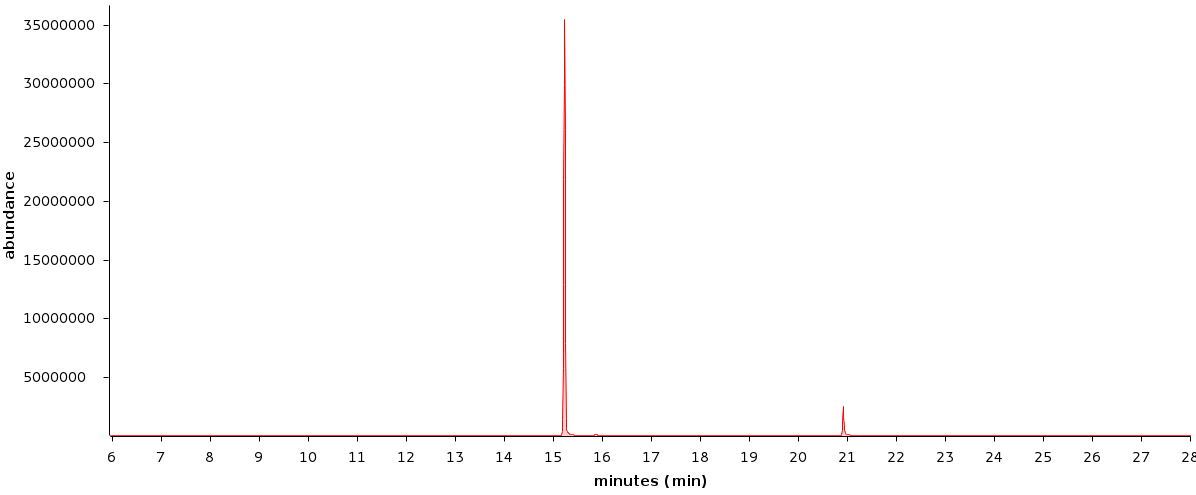
\includegraphics[width=\textwidth]{ig2-12-gcms.png}
\caption[GCMS of Grignard metathesis and quenching reaction.]{GCMS TIC of Grignard metathesis and quenching reaction described in Section~\ref{sec:monomero-regioselettivita}. Product \cmpd+{ig2-9} peak \SI{15.23}{\minute}, area 94~\%; precursor \cmpd+{ig2-10} peak \SI{20.92}{\minute}, area 6~\%.}
\label{fig:ig2-12-gcms}
\end{figure}%

\begin{figure}%ig2-13-gcms
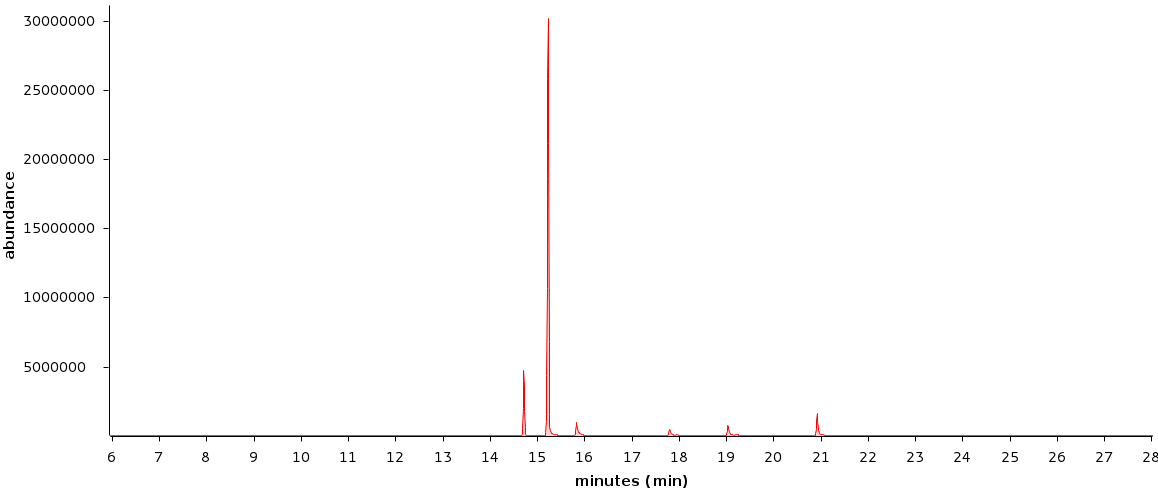
\includegraphics[width=\textwidth]{ig2-13-gcms.png}
\caption[GCMS of Grignard metathesis in presence of lithium chloride and quenching reaction.]{GCMS TIC of Grignard metathesis in presence of lithium chloride and quenching reaction described in Section~\ref{sec:monomero-regioselettivita}. Product \cmpd+{ig2-9} peak \SI{15.22}{\minute}, area 78~\%; precursor \cmpd+{ig2-10} peak \SI{20.91}{\minute}, area 4~\%.}
\label{fig:ig2-13-gcms}
\end{figure}

\FloatBarrier
\clearpage

\FloatBarrier
\clearpage
\section*{Nuclear Magnetic Resonance}

\label{sec:hnmr}

\begin{figure}%ig2-4-nmr-h
\centering
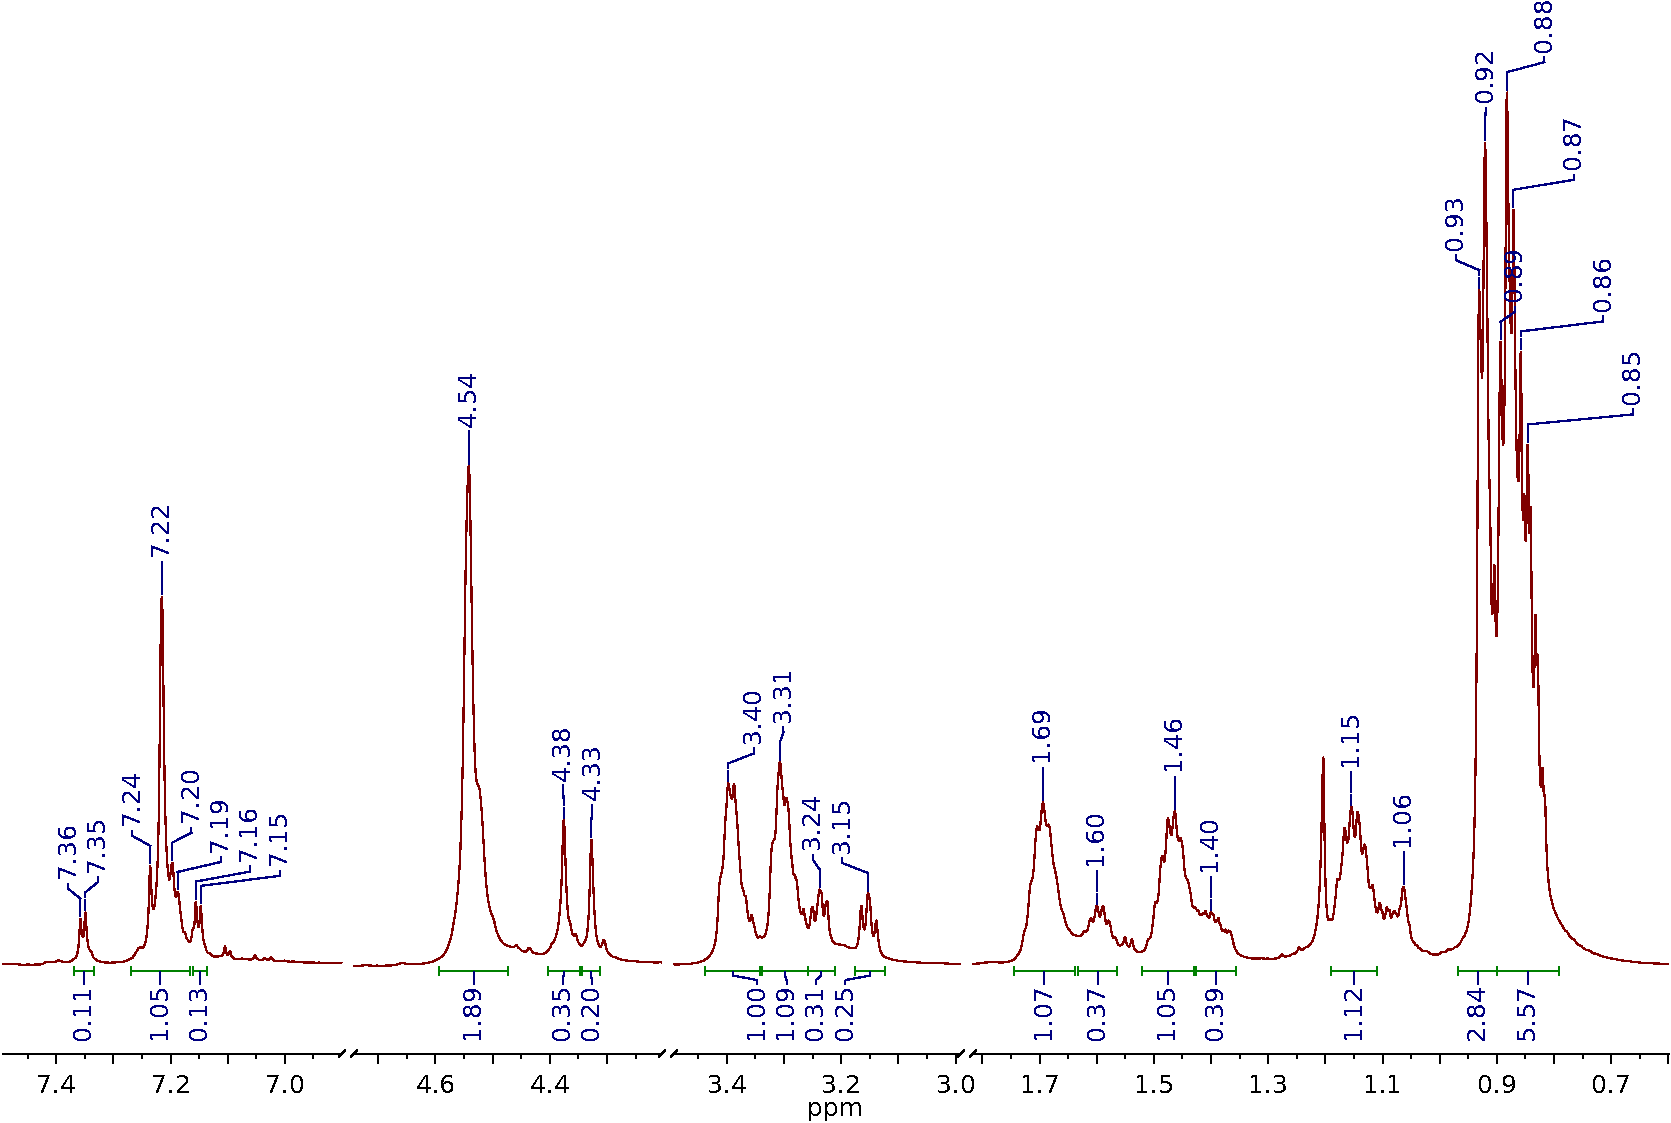
\includegraphics[width=1\textwidth]{ig2-4-nmr-h.pdf}
\caption[{\HNMR} of polymer \cmpd+{ig2-4}.]{{\HNMR} (\SI{600}{\MHz}) of polymer \cmpd+{ig2-4} (\SI{35}{\mg}, \SI{5}{\mm} tube) in \gls{TCE}-d2.}
\label{fig:ig2-4-nmr-h}
\end{figure}

\begin{figure}%ig2-4-nmr-c
\centering
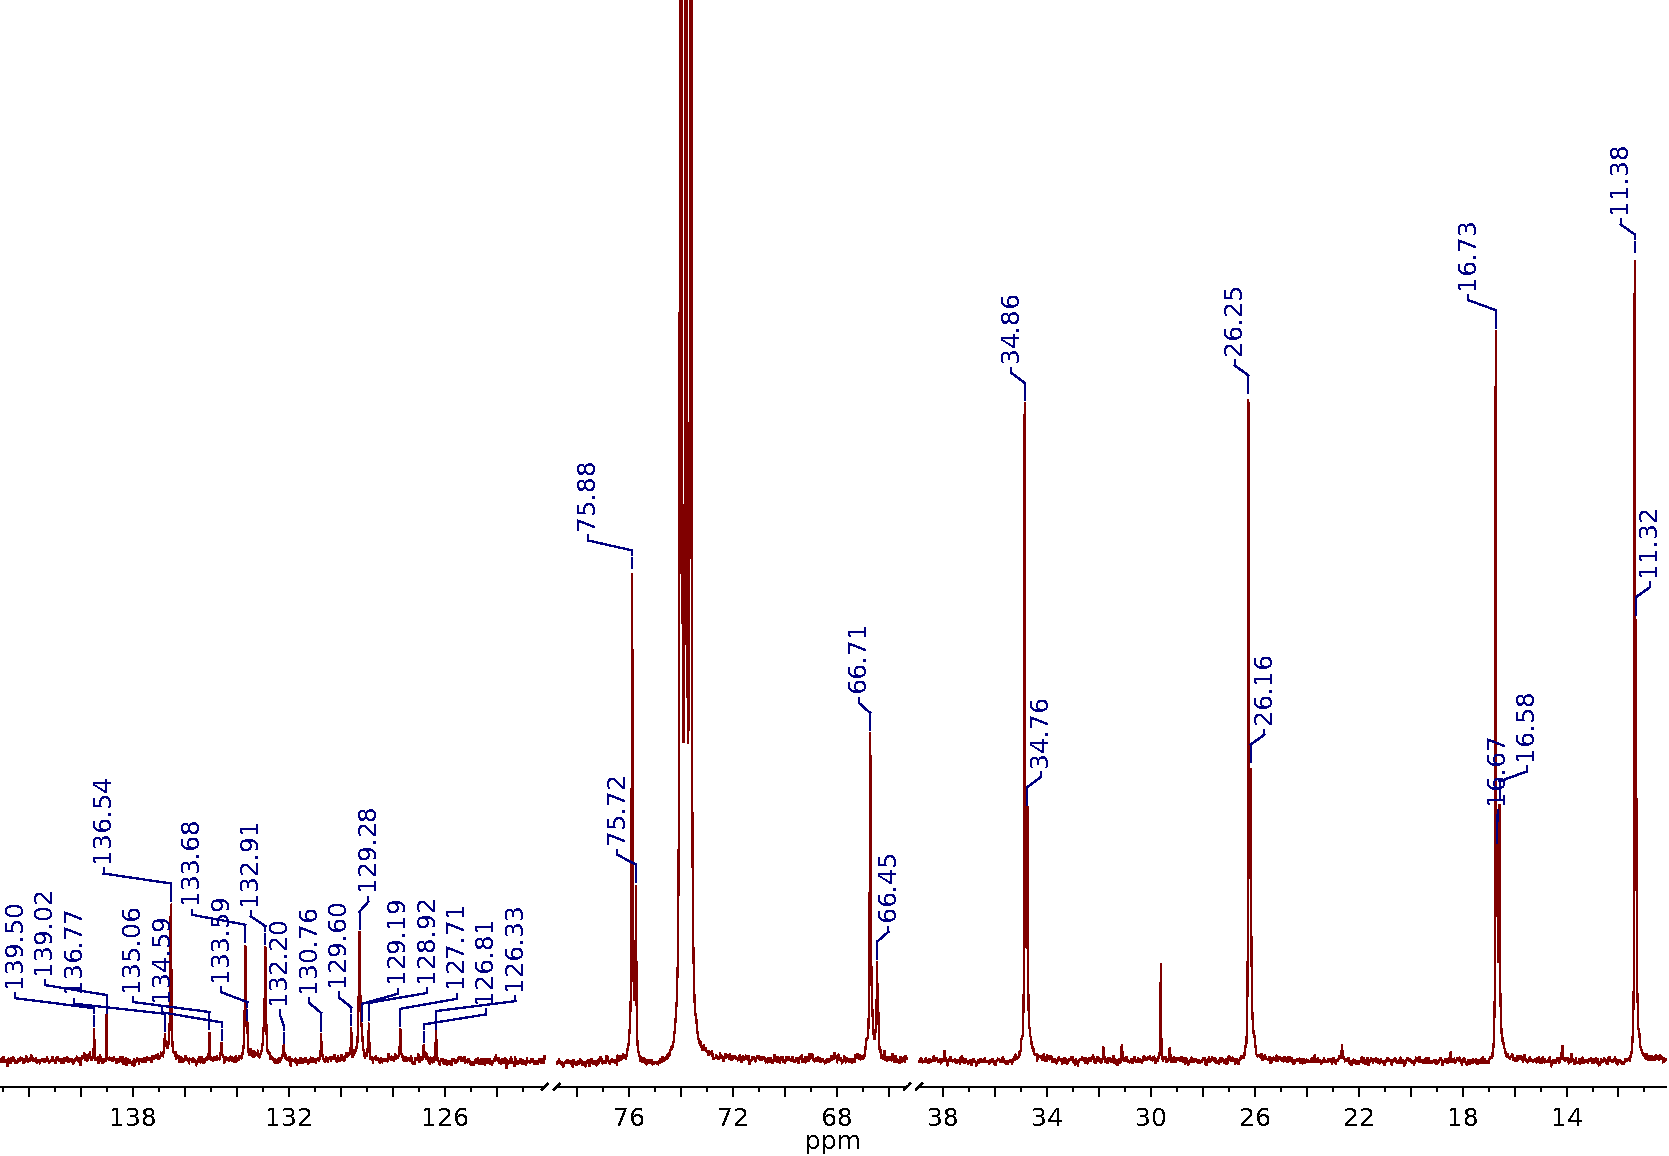
\includegraphics[trim=0 0 0 2.5cm,clip,width=1\textwidth]{ig2-4-nmr-c.pdf}
\caption[{\CNMR} of polymer \cmpd+{ig2-4}.]{{\CNMR} (\SI{150}{\MHz}) of polymer \cmpd+{ig2-4} (\SI{35}{\mg}, \SI{5}{\mm} tube) in \gls{TCE}-d2.}
\label{fig:ig2-4-nmr-c}
\end{figure}

\begin{figure}%ig2-15-nmr-c
\centering
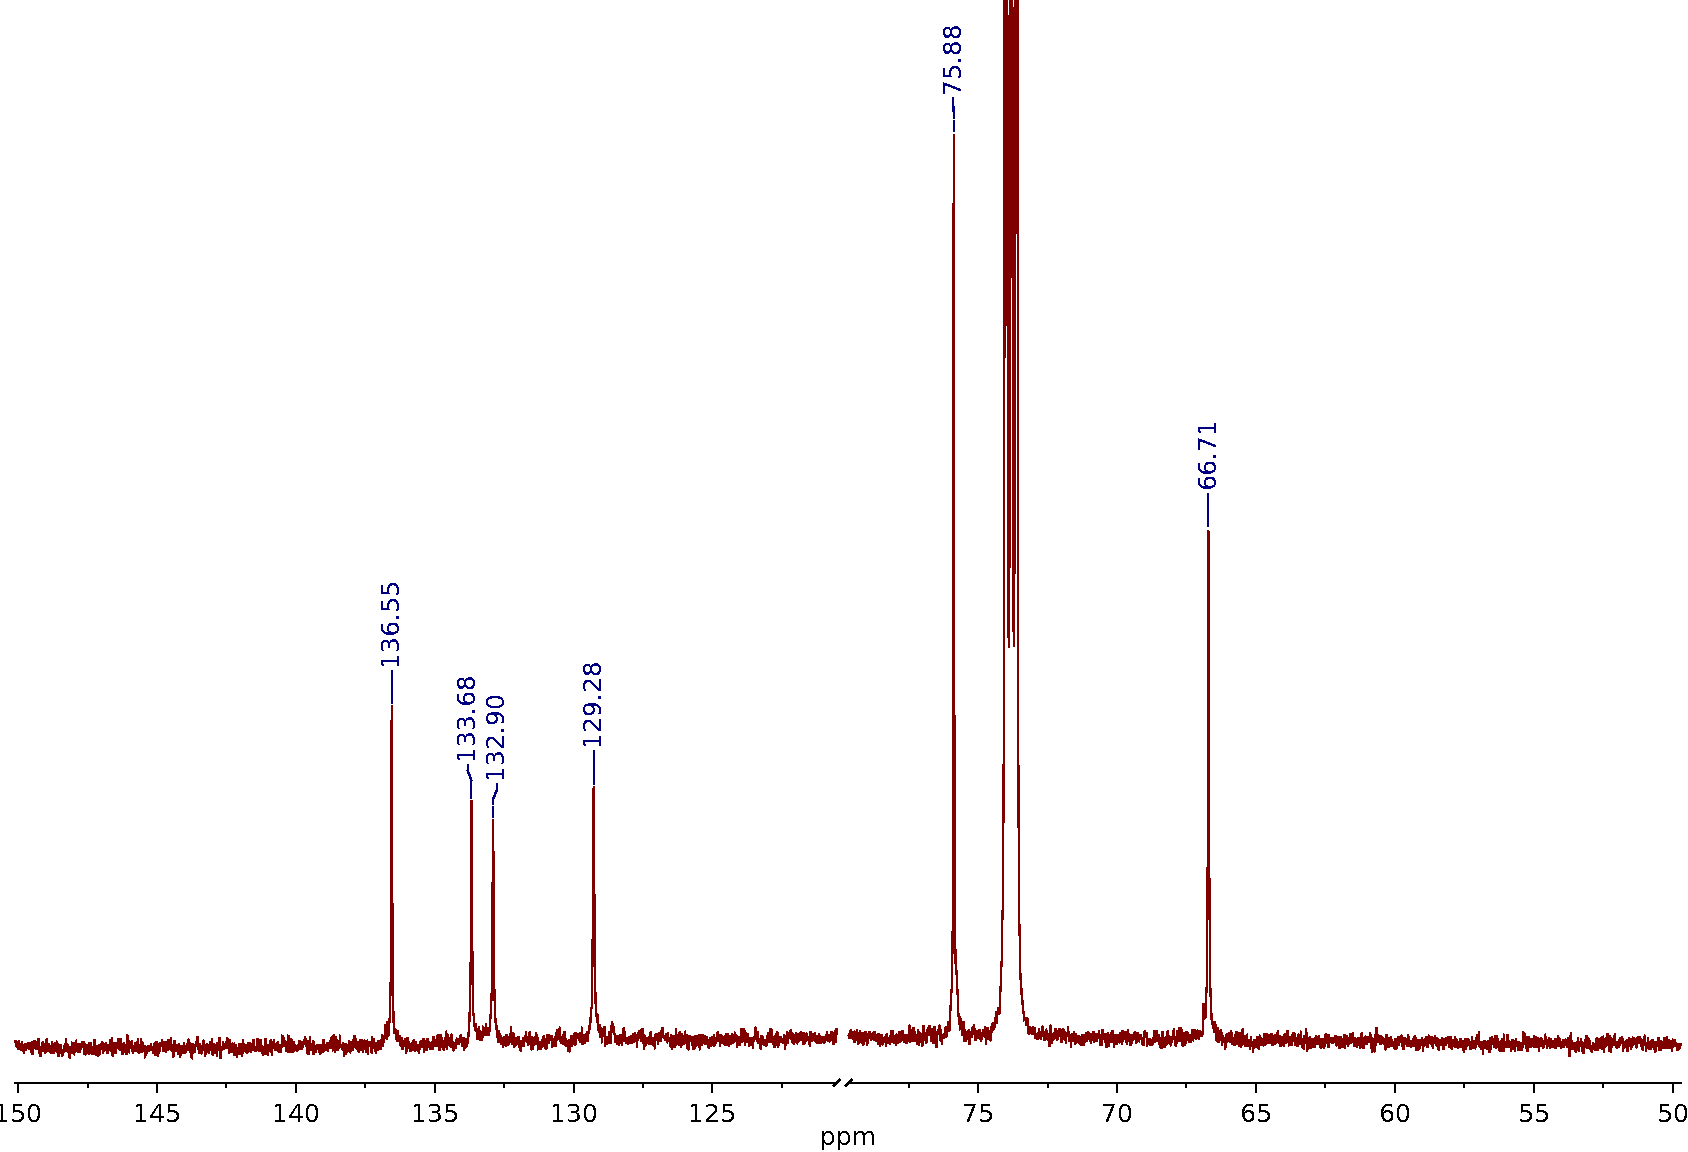
\includegraphics[width=\textwidth]{ig2-15-nmr-c.pdf}
\caption[{\CNMR} of polymer \cmpd+{ig2-15}.]{{\CNMR} (\SI{150}{\MHz}) of polymer \cmpd+{ig2-15} in \gls{TCE}-d2.}
\label{fig:ig2-15-nmr-c}
\end{figure}

\begin{figure}%ig2-8-nmr-h
\centering
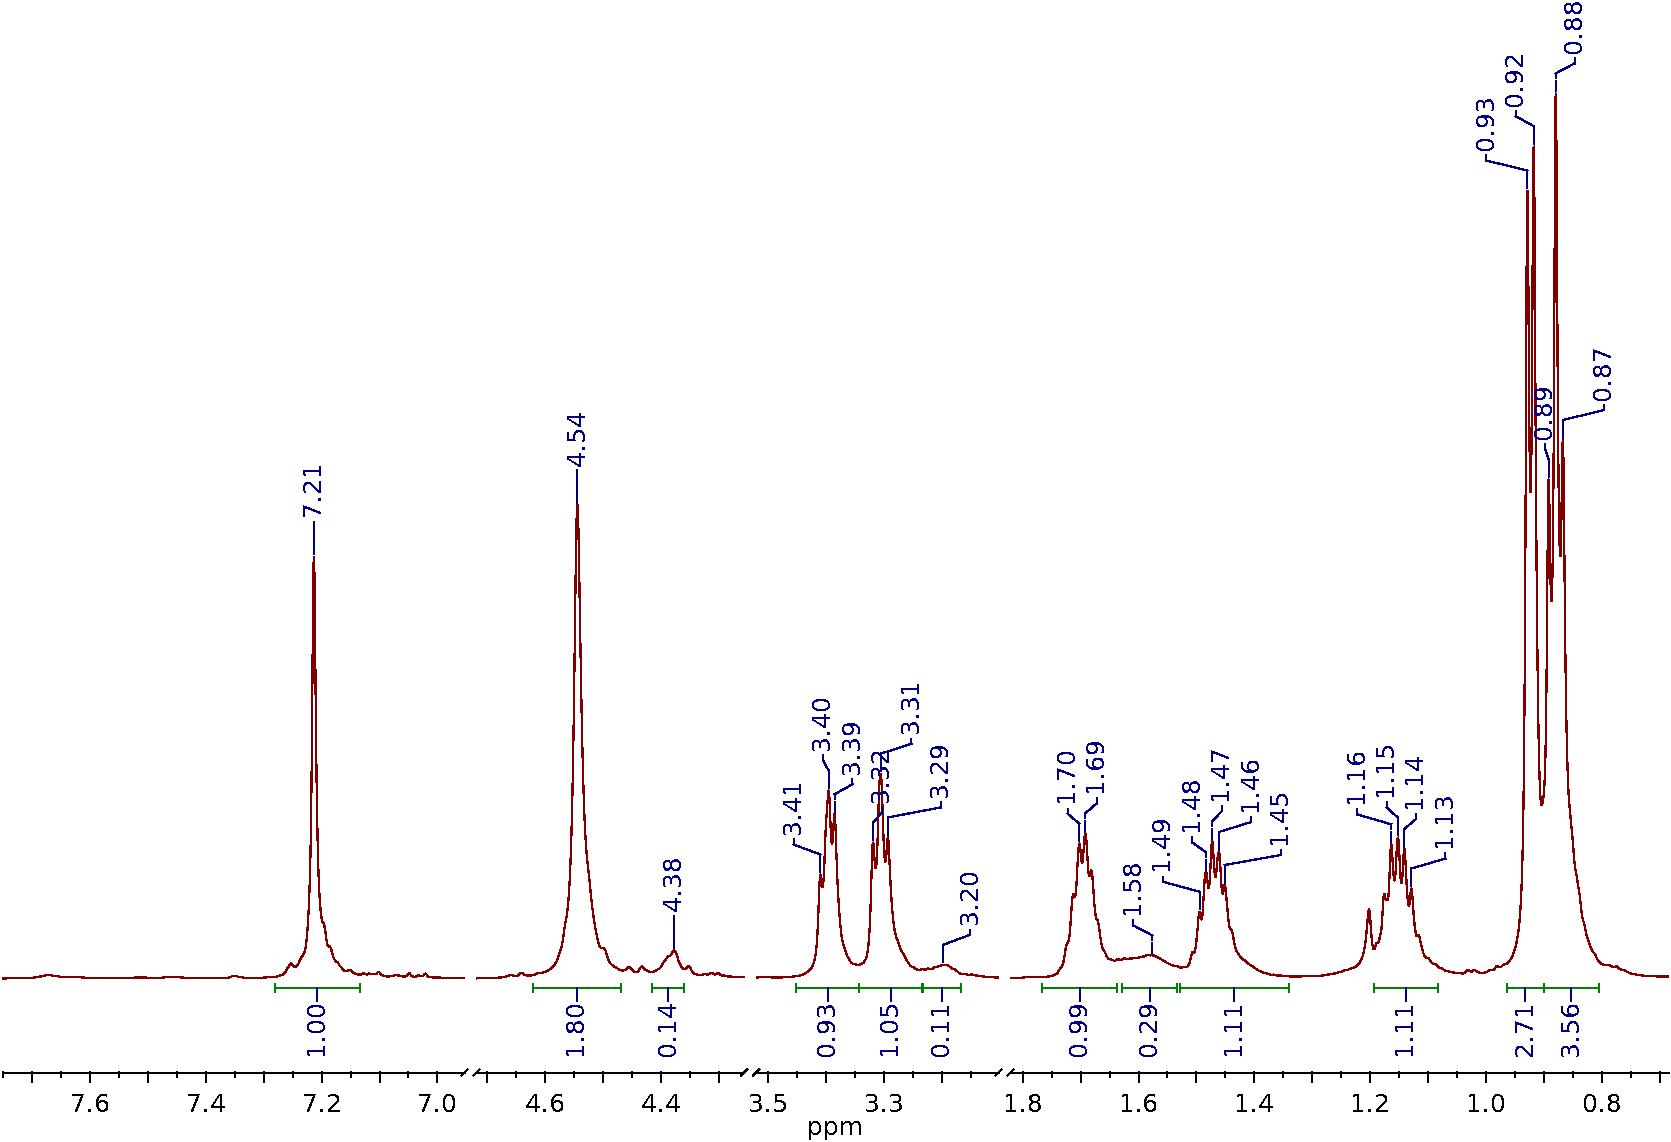
\includegraphics[width=1\textwidth]{ig2-8-nmr-h.pdf}
\caption[{\HNMR} of polymer \cmpd+{ig2-8}.]{{\HNMR} (\SI{600}{\MHz}) of polymer \cmpd+{ig2-8} in \gls{TCE}-d2.}
\label{fig:ig2-8-nmr-h}
\end{figure}

\begin{figure}%ig2-8-nmr-c
\centering
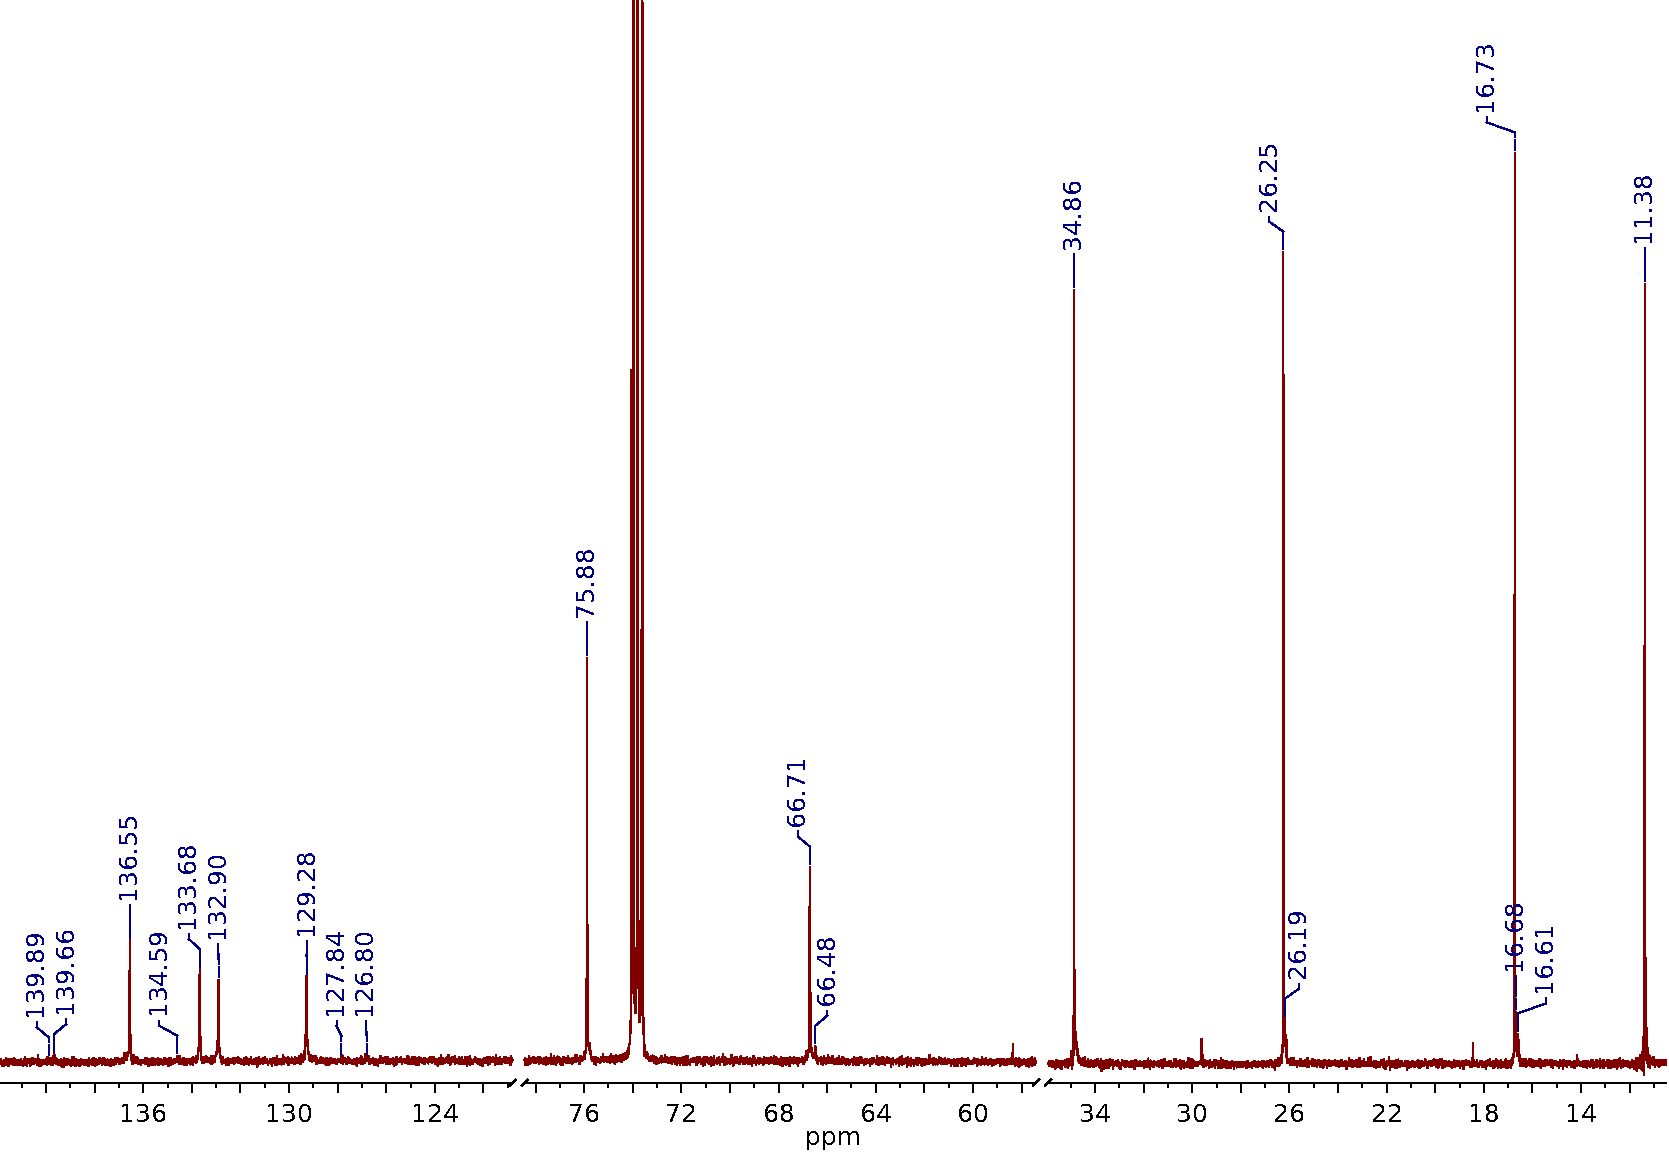
\includegraphics[trim=0 0 0 0.5cm,clip,width=1\textwidth]{ig2-8-nmr-c.pdf}
\caption[{\CNMR} of polymer \cmpd+{ig2-8}.]{{\CNMR} (\SI{150}{\MHz}) of polymer \cmpd+{ig2-8} in \gls{TCE}-d2.}
\label{fig:ig2-8-nmr-c}
\end{figure}

\begin{figure}%ig2-21-nmr-h
\centering
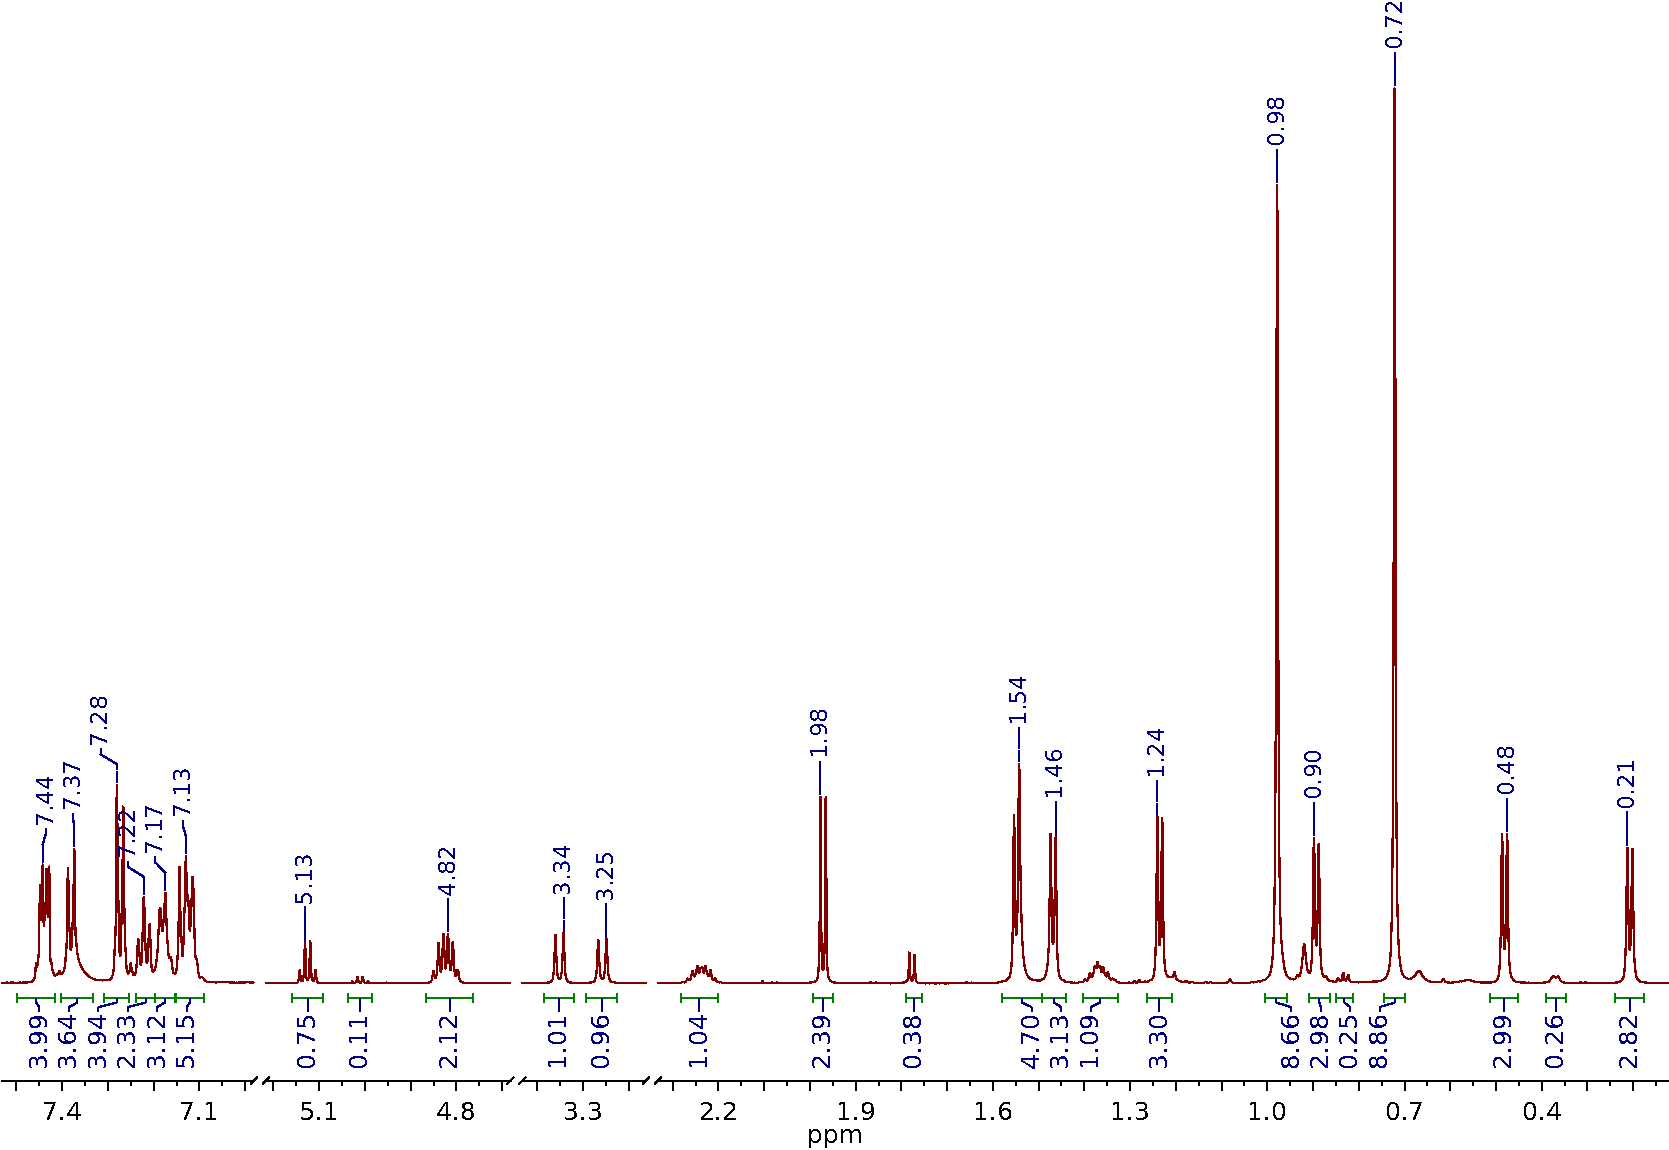
\includegraphics[width=0.95\textwidth]{ig2-21-nmr-h.pdf}
\caption[{\HNMR} of NMRP initiator PhEt-TIPNO \cmpd+{ig2-21}.]{{\HNMR} (\SI{600}{\MHz}) of \gls{NMRP} initiator \gls{BrPhEtTIPNO} \cmpd+{ig2-21} in \gls{TCE}-d2.}
\label{fig:ig2-21-nmr-h}
\end{figure}

\begin{figure}%ig2-19-nmr-h
\centering
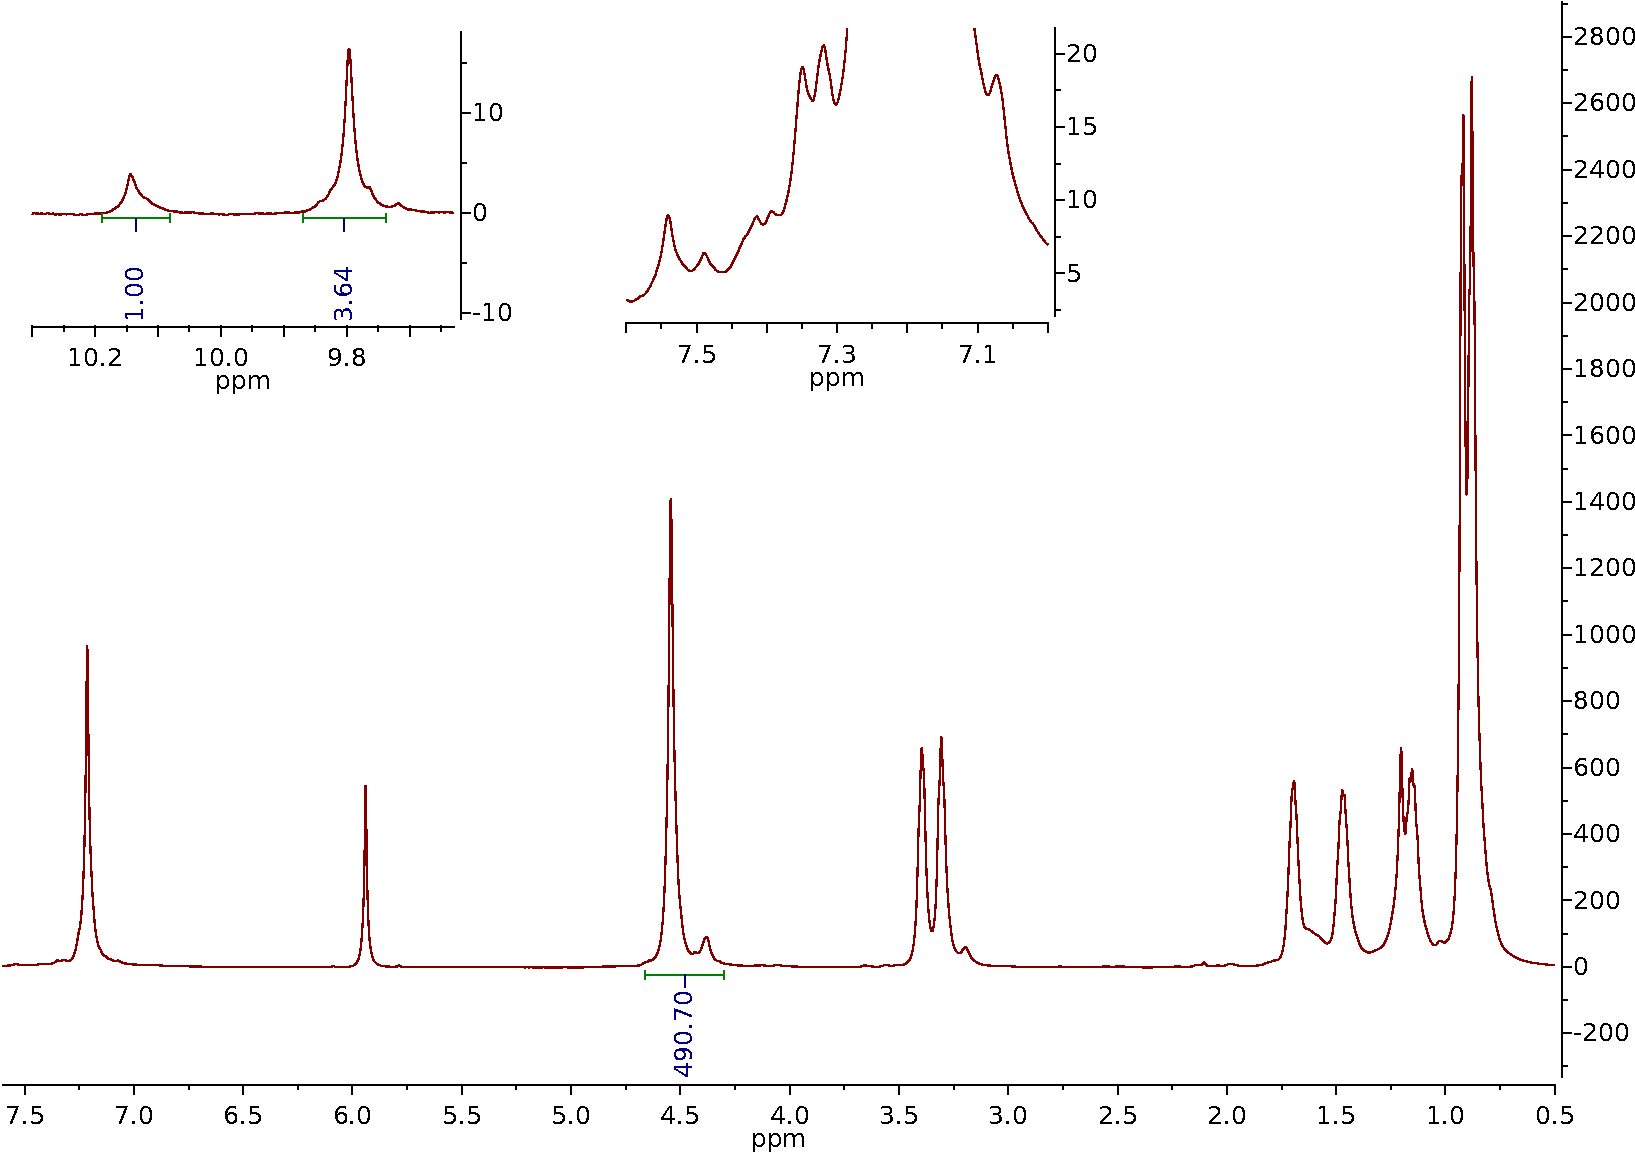
\includegraphics[width=0.95\textwidth]{ig2-19-nmr-h.pdf}
\caption[{\HNMR} of polythiophene-aldehyde \cmpd+{ig2-19}.]{{\HNMR} (\SI{600}{\MHz}) of polythiophene-aldehyde \cmpd+{ig2-19} in \gls{TCE}-d2.}
\label{fig:ig2-19-nmr-h}
\end{figure}

\begin{figure}%ig2-22-nmr-h
\centering
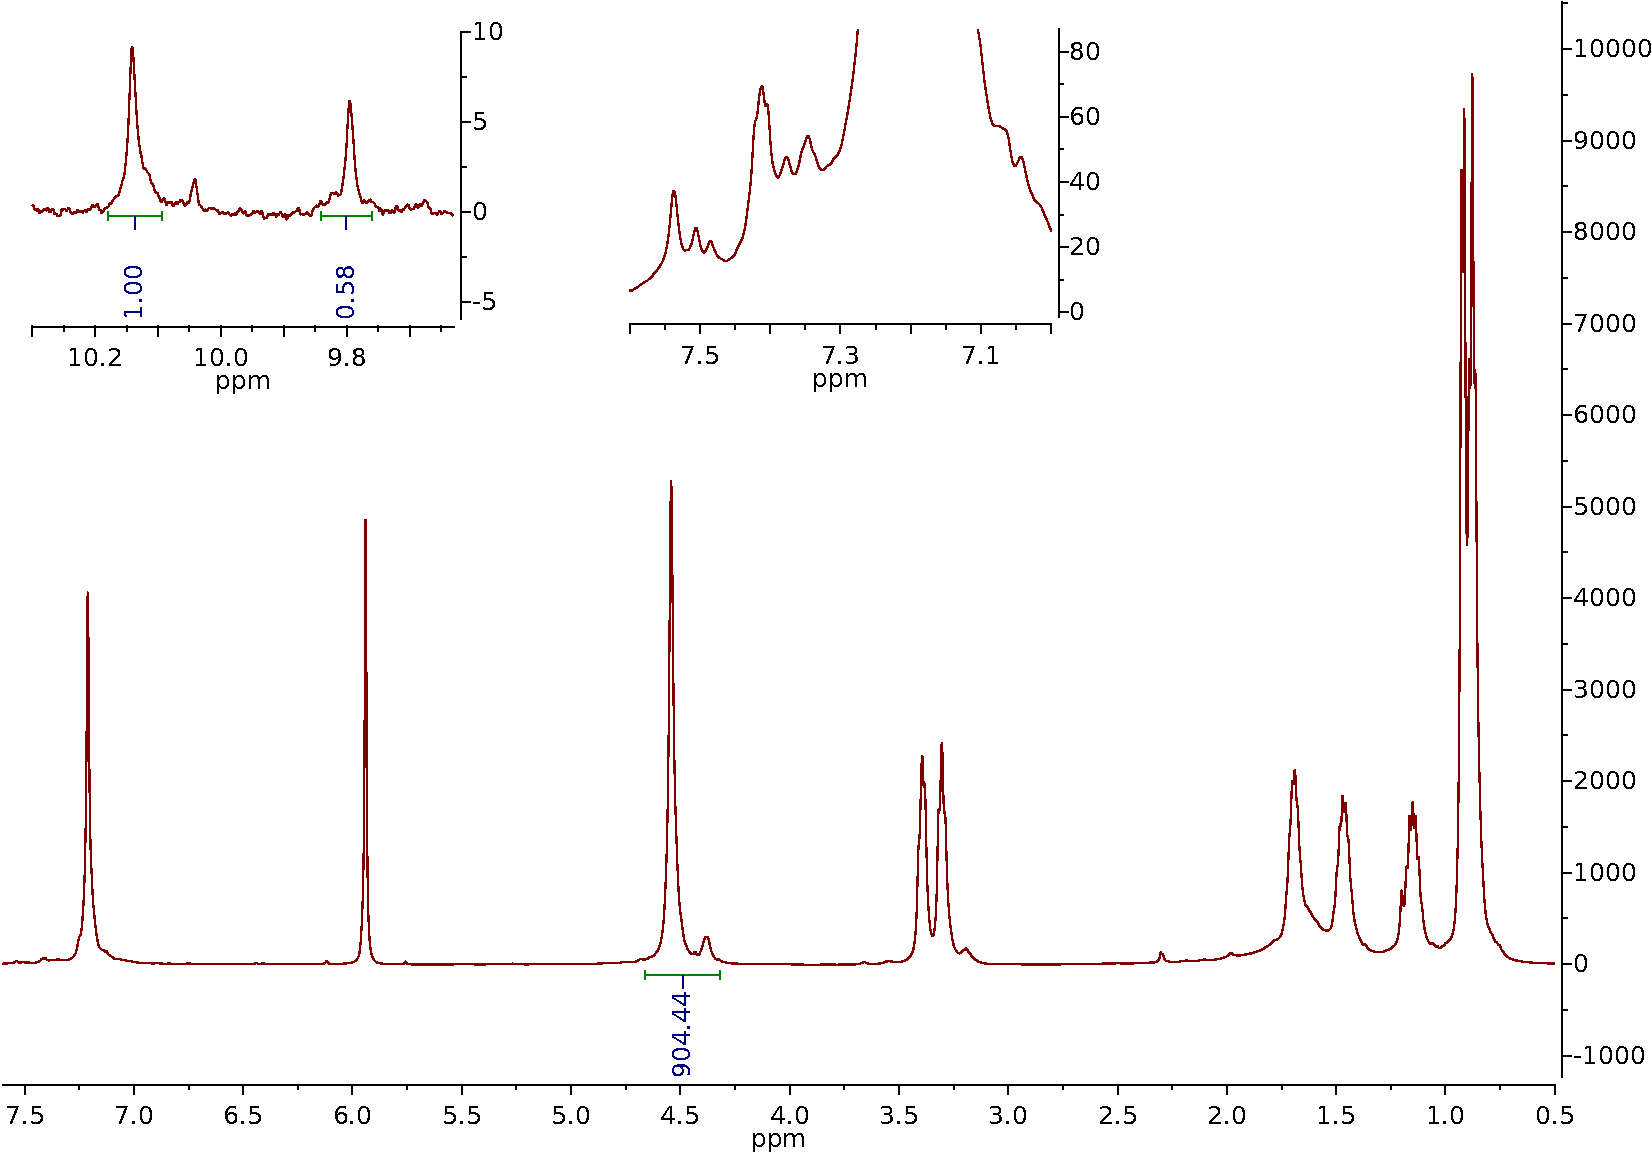
\includegraphics[width=0.95\textwidth]{ig2-22-nmr-h.pdf}
\caption[{\HNMR} of polythiophene-TIPNO \cmpd+{ig2-22}.]{{\HNMR} (\SI{600}{\MHz}) of polythiophene-TIPNO \cmpd+{ig2-22} in \gls{TCE}-d2.}
\label{fig:ig2-22-nmr-h}
\end{figure}

\begin{figure}%sz17-nmr-h-fraz-toluene
\centering
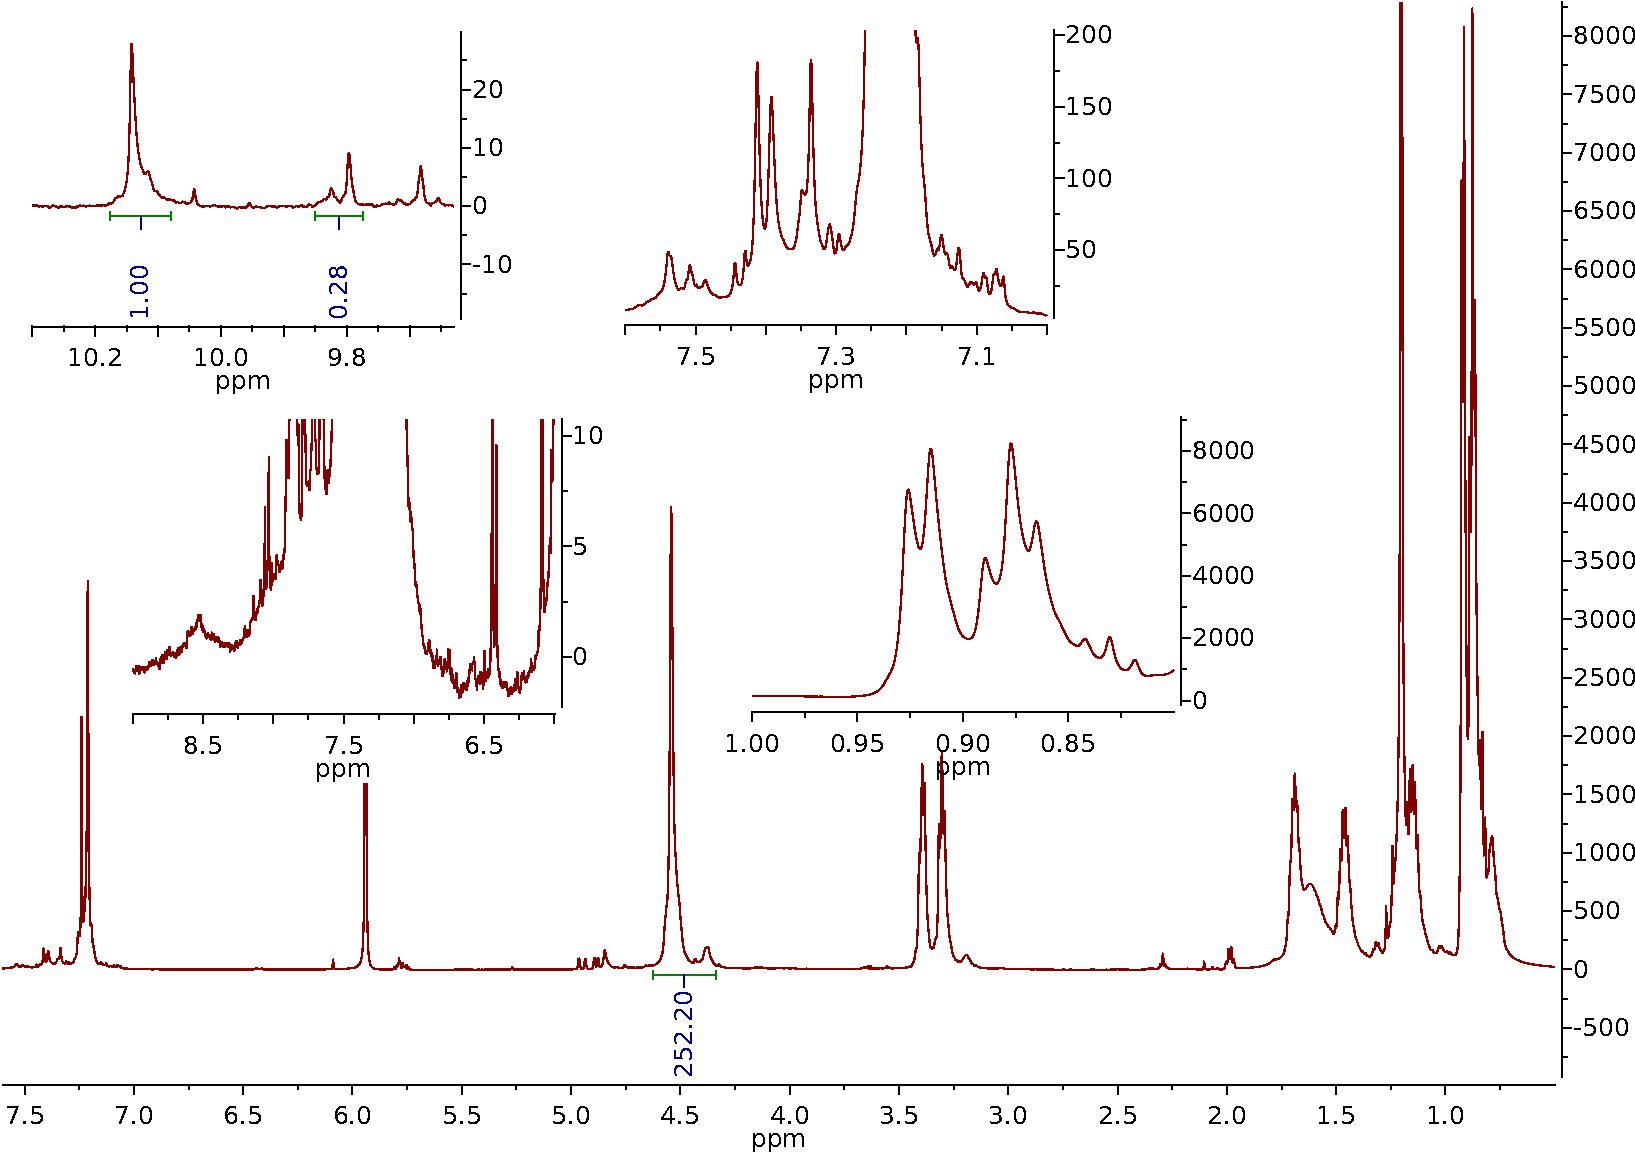
\includegraphics[width=0.95\textwidth]{sz17-nmr-h-fraz-toluene.pdf}
\caption[{\HNMR} of \cmpd+{sz17} washing in toulene.]{{\HNMR} (\SI{600}{\MHz}) of \cmpd+{sz17} washing in toulene in \gls{TCE}-d2.}
\label{fig:sz17-nmr-h-fraz-toluene}
\end{figure}

\begin{figure}%sz17-nmr-h-fraz-cloroformio
\centering
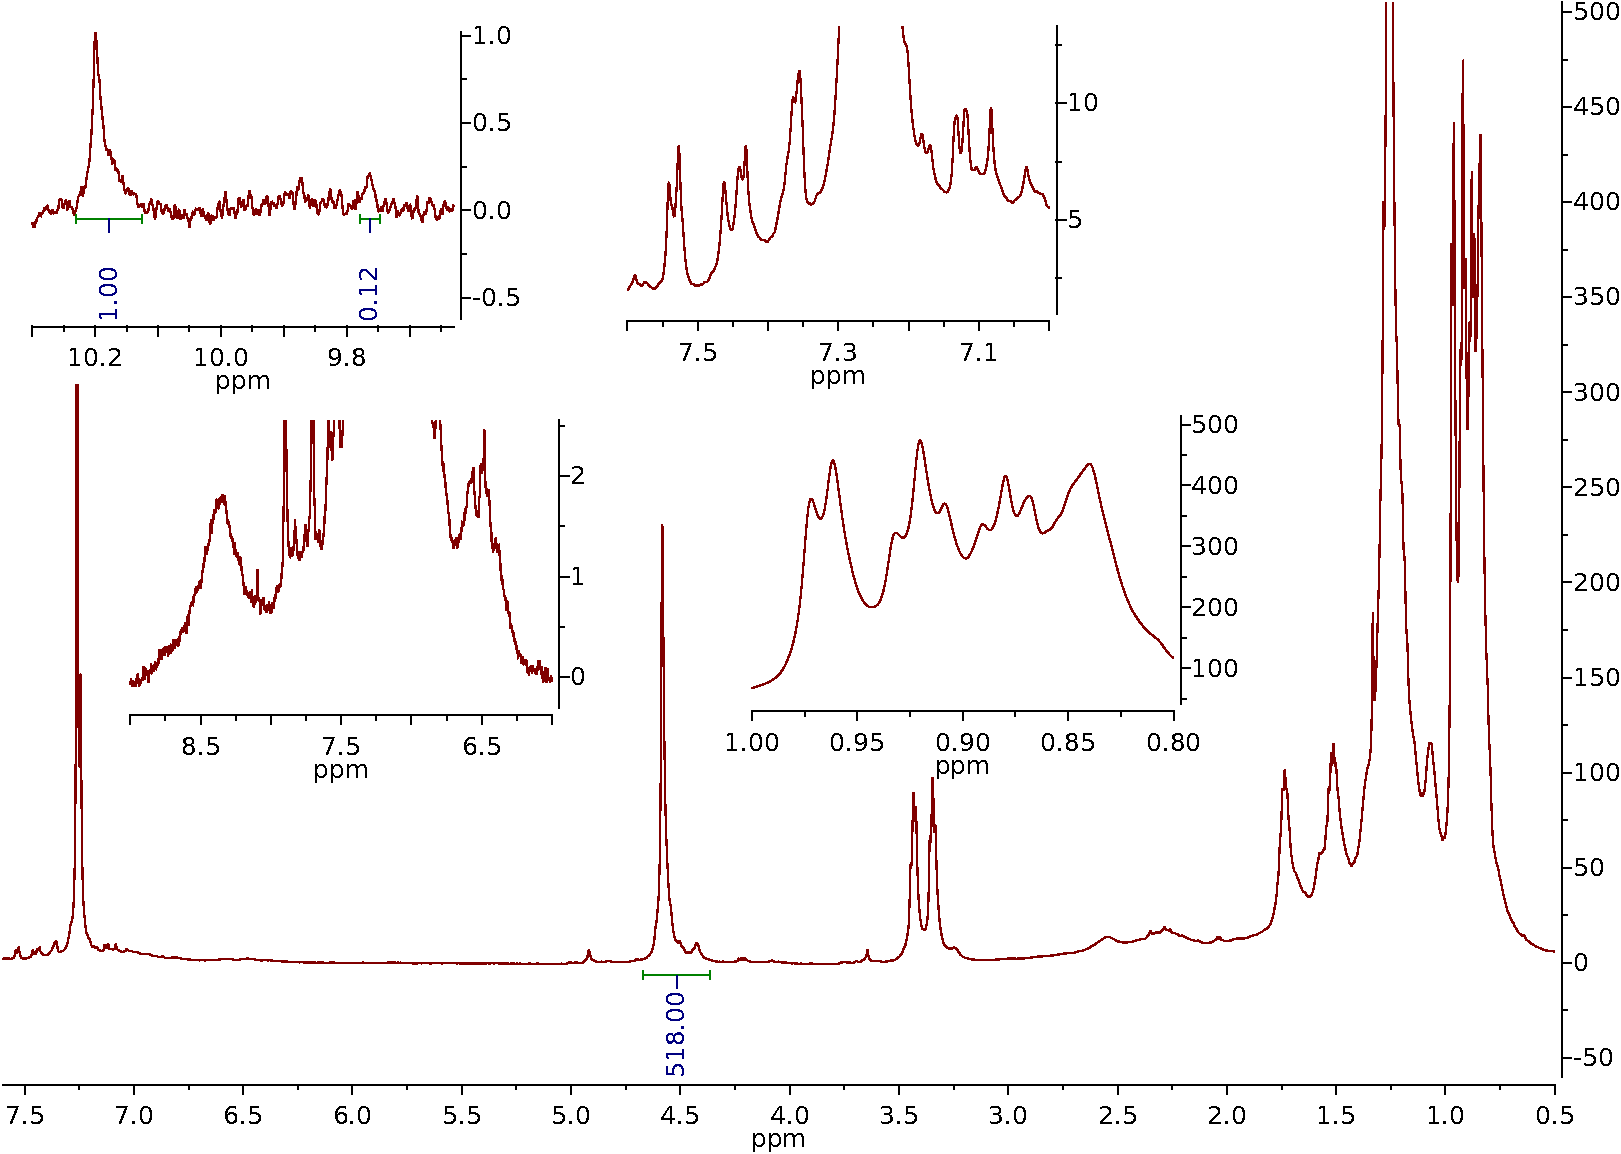
\includegraphics[width=1\textwidth]{sz17-nmr-h-fraz-cloroformio.pdf}
\caption[{\HNMR} of \cmpd+{sz17} purified fraction.]{{\HNMR} (\SI{600}{\MHz}) of \cmpd+{sz17} purified fraction in \ch{CDCl3}.}
\label{fig:sz17-nmr-h-fraz-cloroformio}
\end{figure}

\FloatBarrier
\clearpage

\section*{Mass Spectrometry}

\begin{figure}%ig2-8-maldi-lineare
\begin{tikzpicture}
\begin{axis}[axis x line=bottom,axis y line=left,enlarge x limits=false,enlarge y limits=false,width=1\textwidth,height=6cm,yticklabels={,,},xlabel=Mass-to-charge ratio $m/Q$,ylabel=Intensity (a.\ u.),xmax=14000,cycle list name=linestyles*]
\addplot table {img/results/ig2-8-maldi-lineare-compresso.txt};
\end{axis}
\end{tikzpicture} 

\bigskip

\bigskip

\begin{tikzpicture}
\begin{axis}[axis x line=bottom,axis y line=left,enlarge x limits=false,enlarge y limits=false,width=1\textwidth,height=8cm,yticklabels={,,},xlabel=Mass-to-charge ratio $m/Q$,ylabel=Intensity (a.\ u.),xmin=2720,xmax=2960,cycle list name=linestyles*]
\addplot table {img/results/ig2-8-maldi-lineare-cut.txt};
\end{axis}
\end{tikzpicture} 
\caption[MALDI-TOF MS in linear mode of polymer \cmpd+{ig2-8}.]{\Acrfull{MALDI} in linear mode of polymer \cmpd+{ig2-8}.}
\label{fig:ig2-8-maldi-lineare}
\end{figure}

\FloatBarrier
\clearpage
\section*{Infrared Spectroscopy}

\begin{figure}%ig2-10-ir
\begin{tikzpicture}
\begin{axis}[enlarge x limits=false,enlarge y limits=false,width=1\textwidth,height=7cm,x dir=reverse,xminorgrids=true,xmajorgrids=true,ymajorgrids=true,minor x tick num=4,/pgf/number format/1000 sep={},max space between ticks=80pt,xlabel=Wavenumber (cm$^{-1}$),ylabel=Normalized transmittance (\%)]
\addplot[line width=0.5pt] file {img/spectra/ig2-10-ir.txt};
\end{axis}
\end{tikzpicture}
\caption[FT-IR of pure liquid \cmpd+{ig2-10}.]{FT-IR of pure viscous liquid \cmpd+{ig2-10} on \ch{KBr} disk, discussion in Section~\ref{sec:ir}.}
\label{fig:ig2-10-ir}
\end{figure}

\begin{figure}%ig2-4-ir
\begin{tikzpicture}
\begin{axis}[enlarge x limits=false,enlarge y limits=false,width=1\textwidth,height=7cm,x dir=reverse,xminorgrids=true,xmajorgrids=true,ymajorgrids=true,minor x tick num=4,/pgf/number format/1000 sep={},max space between ticks=80pt,xlabel=Wavenumber (cm$^{-1}$),ylabel=Normalized transmittance (\%)]
\addplot[line width=0.5pt] file {img/spectra/ig2-4-ir.txt};
\end{axis}
\end{tikzpicture}
\caption[FT-IR of polymer \cmpd+{ig2-4}.]{FT-IR of polymer \cmpd+{ig2-4} as a film drop cast from dichloromethane on \ch{KBr} disk, discussion in Section~\ref{sec:ir}.}
\label{fig:ig2-4-ir}
\end{figure}

\begin{figure}%ig2-15-ir
\begin{tikzpicture}
\begin{axis}[enlarge x limits=false,enlarge y limits=false,width=1\textwidth,height=7cm,x dir=reverse,xminorgrids=true,xmajorgrids=true,ymajorgrids=true,minor x tick num=4,/pgf/number format/1000 sep={},max space between ticks=80pt,xlabel=Wavenumber (cm$^{-1}$),ylabel=Normalized transmittance (\%)]
\addplot[line width=0.5pt] file {img/spectra/ig2-15-ir.txt};
\end{axis}
\end{tikzpicture}
\caption[FT-IR of polymer \cmpd+{ig2-15}.]{FT-IR of polymer \cmpd+{ig2-15} as a film drop cast from chloroform on \ch{KBr} disk, discussion in Section~\ref{sec:ir}.}
\label{fig:ig2-15-ir}
\end{figure}

\begin{figure}%ig2-8-ir
\begin{tikzpicture}
\begin{axis}[enlarge x limits=false,enlarge y limits=false,width=1\textwidth,height=7cm,x dir=reverse,xminorgrids=true,xmajorgrids=true,ymajorgrids=true,minor x tick num=4,/pgf/number format/1000 sep={},max space between ticks=80pt,xlabel=Wavenumber (cm$^{-1}$),ylabel=Normalized transmittance (\%)]
\addplot[line width=0.5pt] file {img/spectra/ig2-8-ir.txt};
\end{axis}
\end{tikzpicture}
\caption[FT-IR of polymer \cmpd+{ig2-8}.]{FT-IR of polymer \cmpd+{ig2-8} as a film drop cast from dichloromethane on \ch{KBr} disk, discussion in Section~\ref{sec:ir}.}
\label{fig:ig2-8-ir}
\end{figure}

\FloatBarrier
\clearpage
\section*{Ultraviolet--Visible Spectroscopy}

\begin{figure}%ig2-4-uvvis
\begin{tikzpicture}
\begin{axis}[axis x line=bottom,axis y line=left,yticklabels={,,},enlarge x limits=false,enlarge y limits=false,width=1\textwidth,height=8cm,xlabel=Wavelength (nm),ylabel=Normalized absorbance, xmin=240,xmax=700]
\addplot[line width=0.5pt]
table[y expr=\thisrowno{1}/0.701684] {img/results/ig2-4-uvvis-chcl3.txt};
\addlegendentry{\cmpd+{ig2-4} in \ch{CHCl3}};
\addplot[dashed]
table[y expr=\thisrowno{1}/0.398487-0.3] {img/results/ig2-4-uvvis-chcl3-50-meoh-50.txt};
\addlegendentry{\ch{CHCl3} 50 \% - \ch{MeOH} 50 \%};
\addplot[dashdotted] 
table[y expr=\thisrowno{1}/0.437508-0.7] {img/results/ig2-4-uvvis-chcl3-40-meoh-60.txt};
\addlegendentry{\ch{CHCl3} 40 \% - \ch{MeOH} 60 \%};
\addplot[dotted]
table[y expr=\thisrowno{1}/0.28404-1] {img/results/ig2-4-uvvis-chcl3-30-meoh-70.txt};
\addlegendentry{\ch{CHCl3} 30 \% - \ch{MeOH} 70 \%};
\end{axis}
\end{tikzpicture}
\caption[UV-vis spectra of polymer \cmpd+{ig2-4} in chloroform-methanol mixtures.]{UV-vis spectra of polymer \cmpd+{ig2-4} in chloroform-methanol mixtures.}
\label{fig:ig2-4-uvvis}
\end{figure}

\begin{figure}%ig2-15-uvvis
\begin{tikzpicture}
\begin{axis}[axis x line=bottom,axis y line=left,yticklabels={,,},enlarge x limits=false,enlarge y limits=false,width=1\textwidth,height=8cm,xlabel=Wavelength (nm),ylabel=Normalized absorbance, xmin=240,xmax=600,legend style={at={(0.05,1.25)},anchor=north west,font=\footnotesize}]
\addplot[line width=0.5pt]
table[y expr=\thisrowno{1}/1.04169] {img/results/ig2-15-uvvis-chcl3.txt};
\addlegendentry{\cmpd+{ig2-15} in \ch{CHCl3}};
\addplot[densely dashed]
table[y expr=\thisrowno{1}/1.0759-0.3] {img/results/ig2-15-uvvis-chcl3-50-ch3cn-50.txt};
\addlegendentry{\ch{CHCl3} 50 \% - \ch{CH3CN} 50 \%};
\addplot[dotted]
table[y expr=\thisrowno{1}/0.581413-0.6] {img/results/ig2-15-uvvis-thf.txt};
\addlegendentry{\cmpd+{ig2-15} in \gls{THF}};
\addplot[densely dotted] 
table[y expr=\thisrowno{1}/1.8789-0.9] {img/results/ig2-15-uvvis-thf-55-ch3cn-45.txt};
\addlegendentry{\gls{THF} 55 \% - \ch{CH3CN} 45 \%};
\addplot[dashdotted]
table[y expr=\thisrowno{1}/1.43846-1.25] {img/results/ig2-15-uvvis-thf-70-meoh-30.txt};
\addlegendentry{\gls{THF} 70 \% - \ch{MeOH} 30 \%};
\addplot[dashdotdotted]
table[y expr=\thisrowno{1}/0.983174-1.5] {img/results/ig2-15-uvvis-thf-60-meoh-40.txt};
\addlegendentry{\gls{THF} 60 \% - \ch{MeOH} 40 \%};
\end{axis}
\end{tikzpicture} \caption{UV-vis spectra of polymer \cmpd+{ig2-15} in mixtures of good-poor solvents.}
\label{fig:ig2-15-uvvis}
\end{figure}

\begin{figure}%ig2-8-uvvis-ch3cn
\begin{tikzpicture}
\begin{axis}[axis x line=bottom,axis y line=left,enlarge x limits=false,enlarge y limits=false,width=1\textwidth,height=8cm,xlabel=Wavelength (nm),ylabel=Molar absorptivity (\SI{}{\per\Molar\per\cm}),xmin=240,legend pos=north west,cycle list name=linestyles*]
\addplot table[y expr=\thisrowno{1}/0.0000753] {img/results/ig2-8-uvvis-137-chcl3-for-ch3cn.txt};
\addlegendentry{\cmpd+{ig2-8} in \ch{CHCl3}};
\addplot table[y expr=\thisrowno{1}/0.0000753] {img/results/ig2-8-uvvis-137-chcl3-40-ch3cn-60.txt};
\addlegendentry{\ch{CHCl3} 40 \% - \ch{CH3CN} 60 \%};
\addplot table[y expr=\thisrowno{1}/0.0000753] {img/results/ig2-8-uvvis-137-chcl3-30-ch3cn-70.txt};
\addlegendentry{\ch{CHCl3} 30 \% - \ch{CH3CN} 70 \%};
\addplot table[y expr=\thisrowno{1}/0.0000753] {img/results/ig2-8-uvvis-137-chcl3-20-ch3cn-80.txt};
\addlegendentry{\ch{CHCl3} 20 \% - \ch{CH3CN} 80 \%};
\addplot table[y expr=\thisrowno{1}/0.0000753] {img/results/ig2-8-uvvis-137-chcl3-10-ch3cn-90.txt};
\addlegendentry{\ch{CHCl3} 10 \% - \ch{CH3CN} 90 \%};
\end{axis}
\end{tikzpicture} \caption[UV-vis spectra of polymer \cmpd+{ig2-8} in chloroform-acetonitrile mixtures.]{UV-vis spectra of polymer \cmpd+{ig2-8} in chloroform-acetonitrile mixtures. Concentration \SI{137}{\mg\per\liter}. Pathlength \SI{1}{\mm}. Molar absorptivity is referred to the quantity of thiophene rings; $\epsilon = \mathrm{abs} / ( l (\mathrm{cm}) \cdot c (\mathrm{mol/L}))$.}
\label{fig:ig2-8-uvvis-ch3cn}
\end{figure}

\begin{figure}%ig2-4-uvvis-film
\begin{tikzpicture}
\begin{axis}[axis x line=bottom,axis y line=left,enlarge x limits=false,enlarge y limits=false,width=1\textwidth,height=8cm,xlabel=Wavelength (nm),ylabel=Absorbance,xmin=240,xmax=650,cycle list name=linestyles*]
\addplot table {img/results/ig2-4-uvvis-chcl3.txt};
\addlegendentry{\cmpd+{ig2-4} in \ch{CHCl3}};
\addplot table {img/results/ig2-4-uvvis-chcl3-30-meoh-70.txt};
\addlegendentry{\ch{CHCl3} 30 \% - \ch{MeOH} 70 \%};
\addplot table {img/results/ig2-4-uvvis-spin700-chcl3.txt};
\addlegendentry{spin \SI{700}{\rpm} from \ch{CHCl3}};
\end{axis}
\end{tikzpicture} \caption[UV-vis spectra of polymer \cmpd+{ig2-4} in solution and thin film.]{UV-vis spectra of polymer \cmpd+{ig2-4} in chloroform, in chloroform-methanol solution and thin film spin coated from a chloroform solution at \SI{700}{\rpm}.}
\label{fig:ig2-4-uvvis-film}
\end{figure}

\begin{figure}%ig2-8-uvvis-film
\begin{tikzpicture}
\begin{axis}[axis x line=bottom,axis y line=left,enlarge x limits=false,enlarge y limits=false,width=1\textwidth,height=8cm,xlabel=Wavelength (nm),ylabel=Absorbance,xmin=240,legend style={at={(1,1.2)},anchor=north east,
font=\footnotesize},cycle list name=linestyles*]
\addplot table {img/results/ig2-8-uvvis-cast-chcl3.txt};
\addlegendentry{cast from \ch{CHCl3}};
\addplot table {img/results/ig2-8-uvvis-cast-thf.txt};
\addlegendentry{cast from \gls{THF}};
\addplot table {img/results/ig2-8-uvvis-cast-ch2cl2.txt};
\addlegendentry{cast from \ch{CH2Cl2}};
\addplot table {img/results/ig2-8-uvvis-spin700-chcl3.txt};
\addlegendentry{spin \SI{700}{\rpm} from \ch{CHCl3}};
\addplot table {img/results/ig2-8-uvvis-spin700-thf.txt};
\addlegendentry{spin \SI{700}{\rpm} from \gls{THF}};
\addplot[densely dotted] table {img/results/ig2-8-uvvis-spin1000-chcl3.txt};
\addlegendentry{spin \SI{1000}{\rpm} from \ch{CHCl3}};
\end{axis}
\end{tikzpicture} \caption[UV-vis spectra of polymer \cmpd+{ig2-8} in thin films.]{UV-vis spectra of polymer \cmpd+{ig2-8} in thin films cast and spin coated from various solutions.}
\label{fig:ig2-8-uvvis-film}
\end{figure}

\begin{figure}%ig2-8-uvvis-film-dip
\begin{tikzpicture}
\begin{axis}[axis x line=bottom,axis y line=left,enlarge x limits=false,enlarge y limits=false,width=1\textwidth,height=8cm,xlabel=Wavelength (nm),ylabel=Absorbance,xmin=245,legend style={at={(1,1.2)},anchor=north east,
font=\footnotesize},cycle list name=linestyles*]
\addplot table {img/results/ig2-8-uvvis-spin700-chcl3.txt};
\addlegendentry{spin \SI{700}{\rpm} from \ch{CHCl3}};
\addplot table {img/results/ig2-8-uvvis-spin700-chcl3-dip-pentane.txt};
\addlegendentry{spin \SI{700}{\rpm} from \ch{CHCl3} dip pentane};
\addplot table[y expr=\thisrowno{1}-0.1] {img/results/ig2-8-uvvis-spin700-thf.txt};
\addlegendentry{spin \SI{700}{\rpm} from \gls{THF}};
\addplot table[y expr=\thisrowno{1}-0.1] {img/results/ig2-8-uvvis-spin700-thf-dip-pentane.txt};
\addlegendentry{spin \SI{700}{\rpm} from \gls{THF} dip pentane};
\addplot table[y expr=\thisrowno{1}-0.2] {img/results/ig2-8-uvvis-spin1000-chcl3.txt};
\addlegendentry{spin \SI{1000}{\rpm} from \ch{CHCl3}};
\addplot[densely dotted] table[y expr=\thisrowno{1}-0.2] {img/results/ig2-8-uvvis-spin1000-chcl3-dip-pentane.txt};
\addlegendentry{spin \SI{1000}{\rpm} from \ch{CHCl3} dip pentane};
\end{axis}
\end{tikzpicture} \caption[UV-vis spectra of polymer \cmpd+{ig2-8} in thin films spin coated and dipped in pentane.]{Stacked UV-vis spectra of polymer \cmpd+{ig2-8} in thin film spin coated from various solutions and dipped in pentane.}
\label{fig:ig2-8-uvvis-film-dip}
\end{figure}

\begin{figure}%uvvis-kcl
\begin{tikzpicture}
\begin{axis}[axis x line=bottom,axis y line=left,enlarge x limits=false,enlarge y limits=false,width=1\textwidth,height=8cm,xlabel=Wavelength (nm),ylabel=Absorbance,xmin=240,legend style={at={(1,0.75)},anchor=north east},
cycle list name=linestyles*]
\addplot table {img/results/ig2-4-uvvis-kcl.txt};
\addlegendentry{\cmpd+{ig2-4}};
\addplot table {img/results/ig2-15-uvvis-kcl-3.txt};
\addlegendentry{\cmpd+{ig2-15}};
\addplot table[y expr=(\thisrowno{1}*0.00961)+0.340] {img/results/ig2-8-ht-kcl-2.txt};
\addlegendentry{\cmpd+{ig2-8}};
\end{axis}
\end{tikzpicture} \caption[UV-vis spectra of polymers in \ch{KCl} disks.]{UV-vis spectra of polymers \cmpd+{ig2-4}, \cmpd+{ig2-15} and \cmpd+{ig2-8} in \ch{KCl} disks.}
\label{fig:uvvis-kcl}
\end{figure}
\FloatBarrier
\clearpage
\section*{Photoluminescence}

\begin{figure}%pl-cloroformio
\begin{tikzpicture}
\begin{axis}[axis x line=bottom,axis y line=left,enlarge x limits=false,enlarge y limits=false,width=1\textwidth,height=6cm,xlabel=Wavelength (nm),ylabel=Photoluminescence (a.\ u.),xmin=480,legend style={font=\footnotesize},cycle list name=linestyles*]
\addplot table {img/results/ig2-4-pl-137-chcl3.txt};
\addlegendentry{\cmpd{ig2-4} \SI{137}{\mg\per\liter} in \ch{CHCl3}};
\addplot table {img/results/ig2-4-pl-5480-chcl3.txt};
\addlegendentry{\cmpd{ig2-4} \SI{5.48}{\g\per\liter} in \ch{CHCl3}};
\addplot table {img/results/ig2-15-pl-137-chcl3.txt};
\addlegendentry{\cmpd{ig2-15} \SI{137}{\mg\per\liter} in \ch{CHCl3}};
\addplot table {img/results/ig2-15-pl-5480-chcl3.txt};
\addlegendentry{\cmpd{ig2-15} \SI{5.48}{\g\per\liter} in \ch{CHCl3}};
\addplot table {img/results/ig2-8-pl-137-chcl3.txt};
\addlegendentry{\cmpd{ig2-8} \SI{137}{\mg\per\liter} in \ch{CHCl3}};
\addplot[densely dotted] table {img/results/ig2-8-pl-5480-chcl3.txt};
\addlegendentry{\cmpd{ig2-8} \SI{5.48}{\g\per\liter} in \ch{CHCl3}};
\end{axis}
\end{tikzpicture} \caption[Photoluminescence of polymers in chloroform solution.]{Photoluminescence of polymers \cmpd+{ig2-4}, \cmpd+{ig2-15} and \cmpd+{ig2-8} in chloroform solution.}
\label{fig:pl-cloroformio}
\end{figure}

\begin{figure}%ig2-4-pl
\begin{tikzpicture}
\begin{axis}[axis x line=bottom,axis y line=left,enlarge x limits=false,enlarge y limits=false,width=1\textwidth,height=6cm,xlabel=Wavelength (nm),ylabel=Photoluminescence (a.\ u.),xmin=480,cycle list name=linestyles*]
\addplot table {img/results/ig2-4-pl-137-chcl3.txt};
\addlegendentry{\cmpd{ig2-4} \SI{137}{\mg\per\liter} in \ch{CHCl3}};
\addplot table {img/results/ig2-4-pl-137-chcl3-50-meoh-50.txt};
\addlegendentry{in \ch{CHCl3} 50 \% - \ch{MeOH} 50 \%};
\end{axis}
\end{tikzpicture} \caption{Photoluminescence of polymer \cmpd+{ig2-4} in chloroform-methanol solution.}
\label{fig:ig2-4-pl}
\end{figure}

\FloatBarrier
\clearpage
\section*{Circular Dichroism Spectroscopy}

\begin{figure}%cd-goodsolvent
\begin{tikzpicture}
\begin{axis}[axis x line=bottom,axis y line=left,enlarge x limits=false,enlarge y limits=true,width=1\textwidth,height=6cm,xlabel=Wavelength (nm),ylabel=Circular Dichroism (mdeg),xmin=240,legend pos=north west]
\addplot[line width=0.5pt] table {img/results/ig2-15-cd-thf.txt};
\addlegendentry{\cmpd+{ig2-15} in \gls{THF}};
\addplot[line width=1.7pt] table {img/results/ig2-8-cd-137-chcl3.txt};
\addlegendentry{\cmpd+{ig2-8} in \ch{CHCl3}};
\draw[help lines] (axis cs:240,0) -- (axis cs:600,0);
\end{axis}
\begin{axis}[width=1\textwidth,
enlarge x limits=false,enlarge y limits=true,
axis y line=right,
ylabel=Absorbance,
yticklabels={,,},
axis x line=none,
xmin=240,
height=6cm]
\addplot[line width=0.5pt] table {img/results/ig2-15-ht-thf.txt};
\addplot[line width=1.7pt] table {img/results/ig2-8-ht-137-chcl3.txt};
\end{axis}
\end{tikzpicture} \caption[Circular dichroism of polymer \cmpd+{ig2-15} and \cmpd+{ig2-8} in good solvents solutions.]{Circular dichroism and UV-vis absorbance (as recorder by circular dichroism spectrometer) of polymer \cmpd+{ig2-15} and \cmpd+{ig2-8} in good solvents solutions. Concentration for polymer \cmpd+{ig2-8} was \SI{137}{\mg\per\liter}, for \cmpd+{ig2-15} concentration is unknown. Pathlength \SI{1}{\mm}.}
\label{fig:cd-goodsolvent}
\end{figure}

\begin{figure}%ig2-4-cd-meoh
\begin{tikzpicture}
\begin{axis}[axis x line=bottom,axis y line=left,enlarge x limits=false,enlarge y limits=true,width=1\textwidth,height=6cm,xlabel=Wavelength (nm),ylabel=Molar circular dichroism $\Delta\epsilon$,xmin=240,legend style={at={(0.28,1.05)},anchor=north west,
font=\footnotesize},
cycle list name=linestyles*]
\addplot table[y expr=\thisrowno{1}*0.0806] {img/results/ig2-4-cd-137-chcl3-60-meoh-40.txt};
\addlegendentry{\ch{CHCl3} 60 \% - \ch{MeOH} 40 \%};
\addplot table[y expr=\thisrowno{1}*0.0806] {img/results/ig2-4-cd-137-chcl3-50-meoh-50.txt};
\addlegendentry{\ch{CHCl3} 50 \% - \ch{MeOH} 50 \%};
\addplot table[y expr=\thisrowno{1}*0.0806] {img/results/ig2-4-cd-137-chcl3-40-meoh-60.txt};
\addlegendentry{\ch{CHCl3} 40 \% - \ch{MeOH} 60 \%};
\addplot[line width=1.6pt] table[y expr=\thisrowno{1}*0.0806] {img/results/ig2-4-cd-137-chcl3-20-meoh-80.txt};
\addlegendentry{\ch{CHCl3} 20 \% - \ch{MeOH} 80 \%};
\end{axis}
\end{tikzpicture} \caption[Circular dichroism of polymer \cmpd+{ig2-4} in chloroform-methanol mixtures.]{Circular dichroism of polymer \cmpd+{ig2-4} in chloroform-methanol mixtures. Concentration \SI{137}{\mg\per\liter}. Pathlength \SI{5}{\mm}. Molar circular dichroism is referred to the quantity of thiophene rings; $\Delta\epsilon = \theta (\mathrm{mdeg}) / (32982 \cdot l (\mathrm{cm}) \cdot c (\mathrm{mol/L}))$.}
\label{fig:ig2-4-cd-meoh}
\end{figure}

\begin{figure}%ig2-15-g-thf-ch3cn
\begin{tikzpicture}
\begin{axis}[axis x line=bottom,axis y line=left,enlarge x limits=false,enlarge y limits=true,width=1\textwidth,height=8cm,xlabel=Wavelength (nm),ylabel=Dissymmetry factor $g$,xmin=250,xmax=550,legend pos=north west,cycle list name=linestyles*]
\addplot table {img/results/ig2-15-g-137-thf-50-ch3cn-50.txt};
\addlegendentry{in \gls{THF} 50 \% - \ch{CH3CN} 50 \%};
\addplot table {img/results/ig2-15-g-274-thf-50-ch3cn-50.txt};
\addlegendentry{in \gls{THF} 50 \% - \ch{CH3CN} 50 \% \SI{274}{\mg\per\liter}};
\addplot table {img/results/ig2-15-g-548-thf-50-ch3cn-50.txt};
\addlegendentry{in \gls{THF} 50 \% - \ch{CH3CN} 50 \% \SI{548}{\mg\per\liter}};
\addplot table {img/results/ig2-15-g-137-chcl3-50-meoh-50.txt};
\addlegendentry{in \ch{CHCl3} 50 \% - \ch{MeOH} 50 \%};
\end{axis}
\end{tikzpicture} \caption[Dissymmetry factor of polymer \cmpd+{ig2-15} at various concentrations in THF - \ch{CHCl3}.]{Dissymmetry factor of polymer \cmpd+{ig2-15} in \gls{THF} 50~\% - \ch{CH3CN} 50~\% at various concentrations and comparison with polymer in \ch{CHCl3} 50~\% - \ch{MeOH} 50~\% mixture. Where not specified a concentration of \SI{137}{\mg\per\liter} was used. Pathlength \SI{1}{\mm}.}
\label{fig:ig2-15-g-thf-ch3cn}
\end{figure}

\begin{figure}%ig2-15-cd-anomali
\begin{tikzpicture}
\begin{axis}[axis x line=bottom,axis y line=left,enlarge x limits=false,enlarge y limits=true,width=1\textwidth,height=8cm,xlabel=Wavelength (nm),ylabel=Circular Dichroism (mdeg),xmin=240,legend pos=south west,cycle list name=linestyles*]
\addplot table {img/results/ig2-15-cd-chcl3-30-ch3cn-70-anomalo.txt};
\addlegendentry{in \ch{CHCl3} 30 \% - \ch{CH3CN} 70 \%};
\addplot table {img/results/ig2-15-cd-thf-50-ch3cn-50-anomalo.txt};
\addlegendentry{in \gls{THF} 50 \% - \ch{CH3CN} 50 \%};
\addplot table {img/results/ig2-15-cd-thf-50-ch3cn-50-anomalo-1day.txt};
\addlegendentry{in \gls{THF} 50 \% - \ch{CH3CN} 50 \% \SI{1}{\day}};
\end{axis}
\end{tikzpicture} \caption[Unusual circular dichroism found for polymer \cmpd+{ig2-15}.]{Unusual circular dichroism found for polymer \cmpd+{ig2-15} in chloroform-acetonitrile and tetrahydrofuran-acetonitrile mixture. Concentration not known.}
\label{fig:ig2-15-cd-anomali}
\end{figure}

\begin{figure}%ig2-8-cd-ch3cn
\begin{tikzpicture}
\begin{axis}[axis x line=bottom,axis y line=left,enlarge x limits=false,enlarge y limits=true,width=1\textwidth,height=6cm,xlabel=Wavelength (nm),ylabel=Molar circular dichroism $\Delta\epsilon$,xmin=240,legend pos=north west,cycle list name=linestyles*]
\addplot table[y expr=\thisrowno{1}*0.403] {img/results/ig2-8-cd-137-chcl3-40-ch3cn-60.txt};
\addlegendentry{in \ch{CHCl3} 40 \% - \ch{CH3CN} 60 \%};
\addplot table[y expr=\thisrowno{1}*0.403] {img/results/ig2-8-cd-137-chcl3-30-ch3cn-70.txt};
\addlegendentry{in \ch{CHCl3} 30 \% - \ch{CH3CN} 70 \%};
\addplot table[y expr=\thisrowno{1}*0.403] {img/results/ig2-8-cd-137-chcl3-20-ch3cn-80.txt};
\addlegendentry{in \ch{CHCl3} 20 \% - \ch{CH3CN} 80 \%};
\addplot table[y expr=\thisrowno{1}*0.403] {img/results/ig2-8-cd-137-chcl3-10-ch3cn-90.txt};
\addlegendentry{in \ch{CHCl3} 10 \% - \ch{CH3CN} 90 \%};
\end{axis}
\end{tikzpicture} \caption[Circular dichroism of polymer \cmpd+{ig2-8} in chloroform-acetonitrile.]{Circular dichroism of polymer \cmpd+{ig2-8} in chloroform-acetonitrile mixtures. Concentration \SI{137}{\mg\per\liter}. Pathlength \SI{1}{\mm}.}
\label{fig:ig2-8-cd-ch3cn}
\end{figure}

\begin{figure}%ig2-8-cd-thf-ch3cn
\begin{tikzpicture}
\begin{axis}[axis x line=bottom,axis y line=left,enlarge x limits=false,enlarge y limits=true,width=1\textwidth,height=6cm,xlabel=Wavelength (nm),ylabel=Molar circular dichroism $\Delta\epsilon$,xmin=240,legend pos=north west,cycle list name=linestyles*]
\addplot table[y expr=\thisrowno{1}*0.403] {img/results/ig2-8-cd-137-thf-60-ch3cn-40.txt};
\addlegendentry{in \gls{THF} 60 \% - \ch{CH3CN} 40 \%};
\addplot table[y expr=\thisrowno{1}*0.403] {img/results/ig2-8-cd-137-thf-50-ch3cn-50.txt};
\addlegendentry{in \gls{THF} 50 \% - \ch{CH3CN} 50 \%};
\addplot table[y expr=\thisrowno{1}*0.403] {img/results/ig2-8-cd-137-thf-40-ch3cn-60.txt};
\addlegendentry{in \gls{THF} 40 \% - \ch{CH3CN} 60 \%};
\addplot table[y expr=\thisrowno{1}*0.403] {img/results/ig2-8-cd-137-thf-20-ch3cn-80.txt};
\addlegendentry{in \gls{THF} 20 \% - \ch{CH3CN} 80 \%};
\end{axis}
\end{tikzpicture} \caption[Circular dichroism of polymer \cmpd+{ig2-8} in tetrahydrofuran-acetonitrile.]{Circular dichroism of polymer \cmpd+{ig2-8} in tetrahydrofuran-acetonitrile mixtures. Concentration \SI{137}{\mg\per\liter}. Pathlength \SI{1}{\mm}.}
\label{fig:ig2-8-cd-thf-ch3cn}
\end{figure}

\begin{figure}%ig2-4-cd-film
\begin{tikzpicture}
\begin{axis}[axis x line=bottom,axis y line=left,enlarge x limits=false,enlarge y limits=true,width=1\textwidth,height=6cm,xlabel=Wavelength (nm),ylabel=Dissymmetry factor $g$,xmin=250,xmax=550,legend style={at={(0.2,1)},anchor=north west},
cycle list name=linestyles*]
\addplot table {img/results/ig2-4-g-spin700-chcl3.txt};
\addlegendentry{\cmpd+{ig2-4} spin \SI{700}{\rpm} from \ch{CHCl3}};
\addplot table {img/results/ig2-4-g-137-chcl3-40-meoh-60-5mm.txt};
\addlegendentry{in \ch{CHCl3} 40 \% - \ch{MeOH} 60 \%};
\end{axis}
\end{tikzpicture} \caption[Dissymmetry factor \cmpd+{ig2-4} in thin film spin coated.]{Dissymmetry factor of polymer \cmpd+{ig2-4} in thin film spin coated from chloroform and comparison with chloroform-methanol mixture (rescaled). $g(\lambda) = \Delta\epsilon(\lambda) / \epsilon(\lambda)$.}
\label{fig:ig2-4-cd-film}
\end{figure}

\begin{figure}%ig2-15-cd-film
\begin{tikzpicture}
\begin{axis}[axis x line=bottom,axis y line=left,enlarge x limits=false,enlarge y limits=true,width=1\textwidth,height=6cm,xlabel=Wavelength (nm),ylabel=Dissymmetry factor $g$,xmin=250,xmax=550,legend style={at={(0.25,1)},anchor=north west},
cycle list name=linestyles*]
\addplot table {img/results/ig2-15-g-cast-ch2cl2.txt};
\addlegendentry{\cmpd+{ig2-15} cast from \ch{CH2Cl2}};
\addplot table {img/results/ig2-15-g-137-chcl3-50-meoh-50.txt};
\addlegendentry{in \ch{CHCl3} 50 \% - \ch{MeOH} 50 \%};
\end{axis}
\end{tikzpicture} \caption[Dissymmetry factor of polymer \cmpd+{ig2-15} in thin film cast from dichloromethane.]{Dissymmetry factor of polymer \cmpd+{ig2-15} in thin film cast from dichloromethane and comparison with polymer in chloroform-methanol mixture (rescaled).}
\label{fig:ig2-15-cd-film}
\end{figure}

\begin{figure}%ig2-8-cd-film-dip
\begin{tikzpicture}
\begin{axis}[axis x line=bottom,axis y line=left,enlarge x limits=false,enlarge y limits=true,width=1\textwidth,height=8cm,xlabel=Wavelength (nm),ylabel=Circular Dichroism (mdeg),xmin=240,legend style={at={(0.05,1.4)},anchor=north west,font=\footnotesize},
cycle list name=linestyles*]
\addplot table {img/results/ig2-8-cd-spin700-thf.txt};
\addlegendentry{spin \SI{700}{\rpm} frpm \gls{THF}};
\addplot table {img/results/ig2-8-cd-spin700-thf-dip-pentane.txt};
\addlegendentry{spin \SI{700}{\rpm} frpm \gls{THF} dip pentane};
\addplot table[y expr=\thisrowno{1}-1] {img/results/ig2-8-cd-spin700-chcl3.txt};
\addlegendentry{spin \SI{700}{\rpm} frpm \ch{CHCl3}};
\addplot table[y expr=\thisrowno{1}-1] {img/results/ig2-8-cd-spin700-chcl3-dip-pentane.txt};
\addlegendentry{spin \SI{700}{\rpm} frpm \ch{CHCl3} dip pentane};
\addplot table[y expr=\thisrowno{1}-2] {img/results/ig2-8-cd-spin1000-chcl3.txt};
\addlegendentry{spin \SI{1000}{\rpm} frpm \ch{CHCl3}};
\addplot[densely dotted] table[y expr=\thisrowno{1}-2] {img/results/ig2-8-cd-spin1000-chcl3-dip-pentane.txt};
\addlegendentry{spin \SI{1000}{\rpm} frpm \ch{CHCl3} dip pentane};
\end{axis}
\end{tikzpicture} \caption[Circular dichroism of polymer \cmpd+{ig2-8} spin coated and dipped in pentane.]{Circular dichroism of polymer \cmpd+{ig2-8} in thin film from spin coating and dipping in pentane. Spectra are stacked.}
\label{fig:ig2-8-cd-film-dip}
\end{figure}

\FloatBarrier
\clearpage
\section*{Differential Scanning Calorimetry}

\begin{figure}%ig2-15-dsc
\begin{tikzpicture}
\begin{axis}[axis x line=bottom,axis y line=left,enlarge x limits=false,enlarge y limits=true,width=1\textwidth,height=8cm,yticklabels={,,},xlabel=Sample Temperature (\SI{}{\celsius}),ylabel=Heat Flow,legend style={at={(0.28,1)},anchor=north west},cycle list name=linestyles*]
\addplot table {img/results/ig2-15-dsc-risc1.txt};
\addlegendentry{first heating \SI{20}{\celsius\per\minute}};
\addplot table {img/results/ig2-15-dsc-raff1.txt};
\addlegendentry{cooling \SI{10}{\celsius\per\minute}};
\addplot table {img/results/ig2-15-dsc-risc2.txt};
\addlegendentry{second heating \SI{20}{\celsius\per\minute}};
\end{axis}
\end{tikzpicture} \caption[Differential scanning calorimetry of polymer \cmpd+{ig2-15}.]{Differential scanning calorimetry of polymer \cmpd+{ig2-15} in absence of oxygen.}
\label{fig:ig2-15-dsc}
\end{figure}

\begin{figure}%ig2-8-dsc
\begin{tikzpicture}
\begin{axis}[axis x line=bottom,axis y line=left,enlarge x limits=false,enlarge y limits=true,width=1\textwidth,height=6cm,yticklabels={,,},xlabel=Sample Temperature (\SI{}{\celsius}),ylabel=Heat Flow,ymin=34.7,legend pos=north west,cycle list name=linestyles*]
\addplot table {img/results/ig2-8-dsc-risc1.txt};
\addlegendentry{heating \SI{20}{\celsius\per\minute}};
\addplot table {img/results/ig2-8-dsc-raff1.txt};
\addlegendentry{cooling \SI{10}{\celsius\per\minute}};
\end{axis}
\end{tikzpicture} \caption[Differential scanning calorimetry of polymer \cmpd+{ig2-8}.]{Differential scanning calorimetry of polymer \cmpd+{ig2-8} in absence of oxygen.}
\label{fig:ig2-8-dsc}
\end{figure}

\FloatBarrier
\clearpage
\section*{X--Ray Diffraction}

\begin{figure}%xrd-films
\begin{tikzpicture}
\begin{axis}[axis x line=bottom,axis y line=left,enlarge x limits=false,enlarge y limits=true,width=1\textwidth,height=8cm,xlabel=Degrees $2\theta$,ylabel=Intensity (a.\ u.),legend style={font=\footnotesize},legend pos=north west]
\addplot[line width=0.3pt] table {img/results/ig2-4-xrd-spin700.txt};
\addlegendentry{\cmpd{ig2-4} spin \SI{700}{\rpm}};
\addplot[line width=0.8pt] table[y expr=\thisrowno{1}-30] {img/results/ig2-4-xrd-spin1500.txt};
\addlegendentry{\cmpd{ig2-4} spin \SI{1500}{\rpm}};
\addplot[line width=1.3pt] table[y expr=\thisrowno{1}-60] {img/results/ig2-8-xrd-cast-ch2cl2.txt};
\addlegendentry{\cmpd{ig2-8} cast from \ch{CH2Cl2}};
\addplot[line width=1.8pt] table[y expr=\thisrowno{1}-90] {img/results/ig2-8-xrd-cast-ch2cl2-anneal.txt};
\addlegendentry{\cmpd{ig2-8} cast from \ch{CH2Cl2} and annealed};
\addplot[dotted] table[y expr=\thisrowno{1}-120] {img/results/quartz-xrd.txt};
\addlegendentry{quartz baseline};
\end{axis}
\end{tikzpicture} \caption[X-ray diffraction of polymer \cmpd+{ig2-4} and \cmpd+{ig2-8} thin films]{X-ray diffraction of polymer \cmpd+{ig2-4} and \cmpd+{ig2-8} thin films from spin coating or coating on quartz.}
\label{fig:xrd-films}
\end{figure}

\begin{figure}%xrd-smallangle
\begin{tikzpicture}
\begin{axis}[axis x line=bottom,axis y line=left,enlarge x limits=false,enlarge y limits=true,width=1\textwidth,height=6cm,xlabel=Degrees $2\theta$,ylabel=Intensity (a.\ u.),xmin=0.2,legend pos=north west,cycle list name=linestyles*]
\addplot table {img/results/ig2-8-xrdsmallangle.txt};
\end{axis}
\end{tikzpicture} \caption[Small angle X--ray scattering of polymer \cmpd+{ig2-8} in bulk solid.]{\Acrfull{SAXS} of polymer \cmpd+{ig2-8} in bulk solid.}
\label{fig:xrd-smallangle}
\end{figure}

\vfill
\begin{figure}[bh]
\centering
Ilario Gelmetti - \textit{Master Thesis} - 15 October 2013\\
\medskip 
Synthesis and Characterization of Chiral Polythiophenes.
\bigskip


\includegraphics[width=0.3\textwidth]{img/cc-by-sa.pdf}
\end{figure}
